%% ****** Start of file aiptemplate.tex ****** %
%%
%%   This file is part of the files in the distribution of AIP substyles for REVTeX4.
%%   Version 4.1 of 9 October 2009.
%%
%
% This is a template for producing documents for use with 
% the REVTEX 4.1 document class and the AIP substyles.
% 
% Copy this file to another name and then work on that file.
% That way, you always have this original template file to use.

%\documentclass[aip,graphicx]{revtex4-1}
%\documentclass[aip,reprint]{revtex4-1}

%\usepackage{graphicx}

%\draft % marks overfull lines with a black rule on the right
%\documentclass[pre,aps,floatfix,authordate1-4,twocolumn]{revtex4-1}
%\documentclass[pre,aps,floatfix,authordate1-4]{revtex4-1}

\documentclass[aps,prl,superscriptaddress,twocolumn]{revtex4}



%\documentclass[aps,prl,preprint,groupedaddress]{revtex4}

\usepackage{rotating} 
\usepackage{times}
\usepackage{graphicx}
\usepackage{setspace}
\usepackage{amsmath}
\usepackage{epstopdf}
\usepackage[obeyFinal]{easy-todo}
\usepackage{csquotes}

\begin{document}

% Use the \preprint command to place your local institutional report number 
% on the title page in preprint mode.
% Multiple \preprint commands are allowed.
%\preprint{}

\title{NMRlipids IV: Headgroup \& glycerol backbone structures, and cation binding in bilayers with PS lipids} %Title of paper

% repeat the \author .. \affiliation  etc. as needed
% \email, \thanks, \homepage, \altaffiliation all apply to the current author.
% Explanatory text should go in the []'s, 
% actual e-mail address or url should go in the {}'s for \email and \homepage.
% Please use the appropriate macro for the type of information

% \affiliation command applies to all authors since the last \affiliation command. 
% The \affiliation command should follow the other information.

\author{O. H. Samuli Ollila}
\email[]{samuli.ollila@helsinki.fi}
%\homepage[]{Your web page}
\affiliation{Institute of Organic Chemistry and Biochemistry,
Academy of Sciences of the Czech Republic, 
Prague 6, Czech Republic}
\affiliation{Institute of Biotechnology, University of Helsinki}


% Collaboration name, if desired (requires use of superscriptaddress option in \documentclass). 
% \noaffiliation is required (may also be used with the \author command).
%\collaboration{}
%\noaffiliation

\date{\today}

\begin{abstract}
% insert abstract here
  Primarily measured but also simulated NMR order parameters will be collected also for other than phophatidylcholine
  (these are discussed in NMRlipids I) headgroup. The information will be used to understand structural differences between 
  different lipid molecules in bilayers.
\end{abstract}

%\pacs{}% insert suggested PACS numbers in braces on next line

\maketitle %\maketitle must follow title, authors, abstract and \pacs

% Body of paper goes here. Use proper sectioning commands. 
% References should be done using the \cite, \ref, and \label commands


%\label{}
\section{Introduction}
Phosphatidylserine (PS) is the most common negatively
charged lipid in eykaryotic membranes.
PS lipids compose 8.5\% of total lipid weight of erythrocytes,
but the abundance varies between different organelles up to
25-35\% in plasma membrane \cite{lemmon08,leventis10,li14}.
Despite of the relatively low abundance, PS lipids
are important signaling molecules. They interact with
signaling proteins \cite{leventis10}, regulate
surface charge and protein localization \cite{yeung08}, and
induce protein aggregation \cite{zhao04,gorbenko06}.
Some domains spesifically interact PS lipids,
while others are attracted by general electrostatics and the
binding can be regulated by calcium \cite{leventis10}.
Therefore, the structural details
of lipid headgroups and the details of calcium binding
are crucial for the PS mediated signaling processes.

The structure of PS lipid headgroups and their 
interactions with ions have been studied with
various experimental methods and theoretical techniques \cite{roux90,melcrova16,??}.
However, the consesus has not been reached 
due to the difficulties to interpret the experimental data \cite{??} and
the inaccuracies in simulation models at the
headgroup region \cite{botan15,catte16,ollila16}.
Some studies propose that the negatively charged lipids
attract cations only due to the increase of local concentration
in the vicinity of membranes and that the binding constant of cations is similar
to zwitterionic and negatively charged lipids \cite{seelig90,sinn06,??}.
On the other hand, some studies propose specific binding of calcium directly to PS lipid
headgroups \cite{vernier09,boettcher11,??},
The NMR data proposes that the PS headgroup is more rigid than PC,PE or PG
headgroups, but more detailed interperetation has not been done.

%Details of negatively charged lipids and their interactions
%with ions and proteins have been experimentally analyzed with
%various spectroscopic methods \cite{borle85,macdonald87,roux90,seelig90,pan14,melcrova16,??}
%NMR \cite{seelig90,??}, scattering \cite{pan14,??} and fluorescence spectroscopy
%which are often complemented with classical MD simulations \cite{pan14,melcrova16,??}.


Headgroup and glycerol backbone C-H bond order parameters
calculated from MD simulations have been
recently used to interpret the lipid structures in NMR experiments
and to validate lipid structure and ion binding in simulations of
PC lipid bilayers \cite{botan15,catte16,ollila16,ferreira16}.
In this work we apply this approach to PS lipid headgroup
in order to elucidate the structural details and ion binding
to negatively charged lipids. The results are expected to elucidate
also PS mediated signalling events because 
glycerol backbone and headgroup structure and behaviour are similar
in model membranes and in bacteria \cite{gally81,scherer87,seelig90}.


%In NMRlipids I and II project we were looking for a MD model
%which would correctly reproduce headgroup and glycerol
%backbone structures and cation binding for PC lipid bilayers \cite{botan15,catte16}.
%Here we extend the same goal for lipids with negatively charged PS headgroup.
%Chemical structure of PS headgroup together with other common biological
%lipids is shown in Fig. \ref{lipids}.
\begin{figure}[]
  \centering
  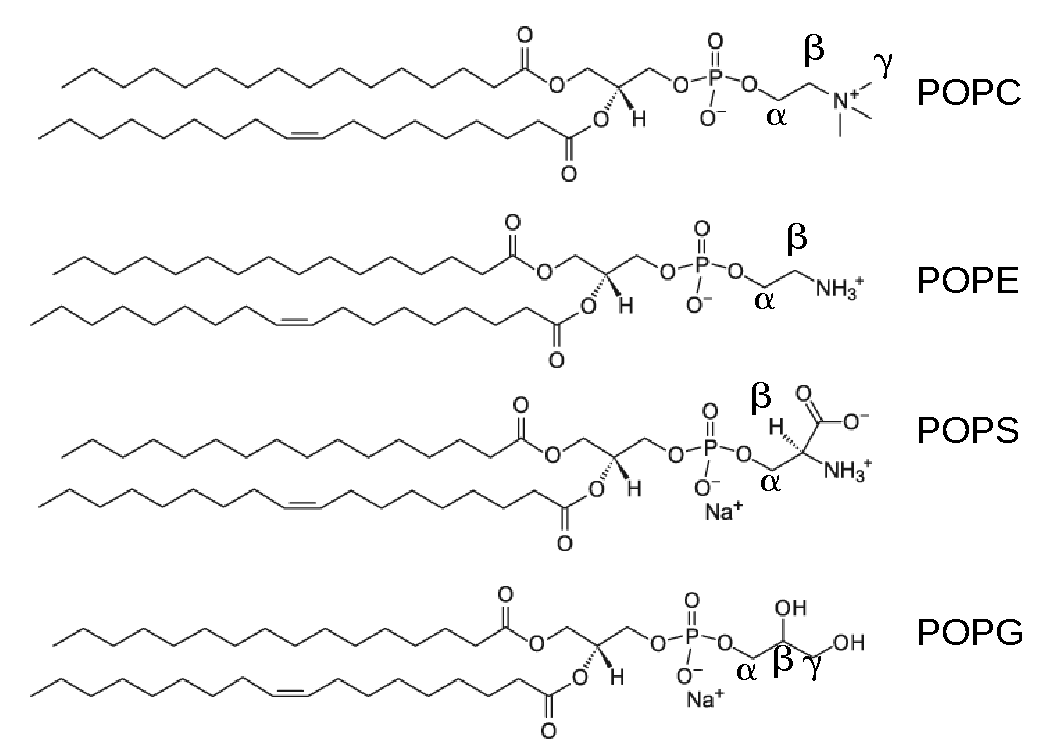
\includegraphics[width=9.0cm]{../Figs/lipids.pdf}
  \caption{\label{lipids}
    Chemical structures and labels for the headgroup carbons.
  }
\end{figure}


%The interpretation of this data and some other results has been that \cite{seelig90}
%\begin{displayquote}
%  {\it ''(i) Ca$^{2+}$ binds to neutral lipids (phosphatidylcholine, phosphatidylethanolamine) and negatively charged lipids
%    (phosphatidylglycerol) with approximately the same binding constant of K = 10-20 M$^{-1}$; \\
%    (ii) the free Ca$^{2+}$
%    concentration at the membrane interface is distinctly enhanced if the membrane carries a negative surface
%    charge, either due to protein or to lipid; \\
%    (iii) increased inter-facial Ca$^{2+}$ also means increased amounts
%    of bound Ca$^{2+}$ at neutral and charged lipids; \\
%    (iv) the actual binding step can be described by a Langmuir
%    adsorption isotherm with a 1 lipid:1 Ca$^{2+}$ stoichiometry, provided the interfacial concentration C$_M$, is
%    used to describe the chemical binding equilibrium.''}
%\end{displayquote}




%Phospholipids containing various polar headgroups and acyl
%chains are essential building blocks of biological membranes.
%Atomistic level structural details of lipids and lipid-ion 
%interactions are considered highly important in several
%biological processes. The lipid structure and ion binding
%can be studied in detail with NMR spectroscopy. However,
%the structural interpretation of NMR data requires usage
%of models. The combination of classical molecular dynamics
%simulations with NMR data, especially with C-H bond
%order parameters, can potentially give atomistic resolution
%interpretation of structure and dynamics of molecules \cite{botan15,ollila16,ferreira16}. 

%Our recent studies concluded that MD models are cabable to
%give structural interpretation for phosphatidylcholine 
%hydrophopic acyl chain region, while hydrophilic headgrop, glycerol 
%backbone and cation binding posed a major challenge for current
%force fields \cite{botan15,ollila16,catte16,ferreira16}. 
%These conclusions were reached by reviewing extensively 
%available experimental data from various sources and using
%NMRlipids Open Collaboration project to collect massive 
%amount of simulation data \cite{botan15,catte16}.

%Here we apply the same approach in search of MD simulation
%models which would reproduce glycerol backbone and 
%headgroup structures of lipids with PE, PG and PS headgroups.  
%In addition, we attempt to find a MD simulation model
%that would be able to correctly describe cation binding in
%bilayer containing negatively charged PG and PS lipids.


%Several MD simulation models have succesfully described 
%acyl chain structures and their qaulitative changes in different
%conditions for phosphatidylcholine lipids (for review see \cite{ollila16}).
%However, the current simulation models were not found to be accurate
%enough for full structural interpretation of phosphatidylcholine headgroup and
%glycerol backbone \cite{botan15}. Also Na$ +$  binding affinities
%were found to be significantly overestimated in several models and 
%none of the available models was able to Ca$2+$ 

\section{Methods}

\subsection{Solid state NMR experiments}
The experimental protocol is the same used in Ref. \citenum{ferreira16}.
\todo{Some basic details should be given.}

\subsection{Molecular dynamics simulations}
Molecular dynamics simulation data was collected with Open Collaboration method.
The simulated systems are listed in Table \ref{IONsystems}.
The simulation details are in SI or in references in the table.
\begin{table*}[!htb]
%\begin{sidewaystable*}[!p]
\centering
\caption{List of MD simulations. The salt concentrations calculated as 
   [salt]=N$_{\rm c} \times$[water]\,/\,N$_{\rm w}$, where [water]\,=\,55.5~M.
   CKP1 referes to the version with Berger/chiu NH3 charges compatible with Berger
   and CKP2 to the version with more Gromos compatible version.
   %   these correspond the concentrations reported in the experiments by Akutsu et al.~\cite{akutsu81}.
   %   The lipid force fields named as in our previous work~\cite{botan15}.
}\label{IONsystems}
%begin{minipage}[t]{\textwidth}
\begin{tabular}{l c c r r r r r r c c}
  %\hline
  % some footnotes are not visible in typeset-MS (pdf)
 lipid/counter-ions & force field for lipids / ions & NaCl (mM) & CaCl$_2$\,(mM) &  \footnote{Number of lipid molecules with largest mole fraction}N$_{\rm l}$   &  \footnote{Number of water molecules}N$_{\rm w}$   & \footnote{Number of additional cations}N$_{\rm c}$  & \footnote{Simulation temperature}T (K)  & \footnote{Total simulation time}t$_{{\rm sim}}$(ns) & \footnote{Time used for analysis}t$_{{\rm anal}}$ (ns) &   \footnote{Reference for simulation files}files\\
  \hline
    DOPS/Na$^+$  & CHARMM36 \cite{??}  \todoi{Correct citation for CHARMM DOPS}      &0 & 0 & 128 & 4480 & 0  & 303  & 500 & 100 & \cite{charmm36DOPS303K} \\
    DOPS/Na$^+$  & CHARMM36ua \cite{??} \todoi{Correct citation for CHARMMua DOPS}        &0 & 0        & 128 & 4480 & 0  & 303  & 500 & 100 & \cite{charmm36uaDOPS303K} \\
    DOPS/Na$^+$  & Slipids \cite{jambeck13}        &0 & 0        & 128 	& 4480  & 0  & 303  & 500 & 100 & \cite{slipidsDOPS303K} \\
    DOPS/Na$^+$  & Slipids \cite{jambeck13}        &0 & 0        & 288 	& 11232 & 0  & 303  & 200 & 100 & \cite{slipidsDOPSfiles} \\
    DOPS/Na$^+$  & Berger \cite{mukhopadhyay04}    &0 & 0        & 128  & 4480  & 0  & 303  & 500 & 100 & \cite{bergerDOPS303K} \\
    DOPS/Na$^+$  & GROMOS-CKP1 \cite{??} \todoi{Correct citation(s) for CKP.} &0 & 0  & 128 & 4480 & 0  & 303  & 500 & 100 & \cite{ckp1DOPS303K} \\
    DOPS/Na$^+$  & GROMOS-CKP2 \cite{??} \todoi{Correct citation(s) for CKP.} &0 & 0  & 128 & 4480 & 0  & 303  & 500 & 100 & \cite{ckp2DOPS303K} \\
    DOPS/Na$^+$  & lipid17 \cite{gould18}          &0 & 0        & ?    & ?   & ?  & ?  & ? & ? & \cite{??} \\
    \hline
    POPS/Na$^+$  & CHARMM36 \cite{??} \todoi{Correct citation for CHARMM POPS}&0 & 0 & 128 & 4480 & 0  & 298  & 500 & 100 & \cite{charmm36POPS298K} \\
    POPS/K$^+$   & CHARMM36 \cite{??} \todoi{Correct citation for CHARMM POPS}&0 & 0 & 128 & 4480 & 0  & 298  & 500 & 100 & \cite{charmm36POPS298Kpotassium} \\
    POPS/Na$^+$  & CHARMM36ua \cite{??} \todoi{Correct citation for CHARMMua DOPS}  &0 & 0 & 128 & 4480 & 0  & 298  & 500 & 100 & \cite{charmm36uaPOPS298K} \\
    POPS/Na$^+$  & Slipids \cite{jambeck13}        &0 & 0        & 128 & 4480 & 0  & 298  & 500 & 100 & \cite{slipidsPOPS298K} \\
    POPS/Na$^+$  & Berger \cite{??}        &0 & 0        & 128 & 4480 & 0  & 298  & 500 & 100 & \cite{bergerPOPS298K} \\
    POPS/Na$^+$  & MacRog \cite{maciejewski14}  &0 & 0        & 128 & 5120 & 0  & 298  & 200 & 100 & \cite{macrogPOPS298K} \\
    POPS/Na$^+$  & GROMOS-CKP1 \cite{??} \todoi{Correct citation(s) for CKP.} &0 & 0  & 128 & 4480 & 0  & 298  & 500 & 100 & \cite{ckp1POPS303K} \\
    POPS/Na$^+$  & GROMOS-CKP2 \cite{??} \todoi{Correct citation(s) for CKP.} &0 & 0  & 128 & 4480 & 0  & 298  & 500 & 100 & \cite{ckp2POPS303K} \\
    POPS/Na$^+$  & lipid17 \cite{gould18}  &0 & 0  & ? & ? & ? & ? & ? & ? & ? \\
    \hline
    POPC:POPS (5:1)/K$^+$  & CHARMM36 \cite{klauda10,??} \todoi{Correct citation for CHARMM POPS}        &0 & 0        & 110:22	   		& 4935 & 0  & 298  & 100 & 100 \todoi{Equilibration?} & \cite{charmm36pops+83popcT298K}  \\
%    \hline
%    POPG/Na$^+$  & CHARMM36 \cite{??} \todoi{Correct citation for CHARMM POPG}        &0 & 0        & ? 			   		& ? & 0  & ?  & ? & ? & \cite{??}
%    \todoi{Details to be filled and data to be uploaded in Zenodo by Ollila.}  \\
%    POPG/Na$^+$  & Slipids \cite{jambeck13}     &0 & 0        & 288 			   		& 10664 & 0  & 298  & 250 & 100 & \cite{slipidsPOPGfiles} \\
%    \hline
%    DPPG/Na$^+$  & Slipids \cite{jambeck13}     &0 & 0        & 288 			   		& 11232 & 0  & 314  & 200 & 100 & \cite{slipidsDPPGfiles} \\
%    DPPG/Na$^+$  & Slipids \cite{jambeck13}     &0 & 0        & 288 			   		& 11232 & 0  & 298  & 400 & 100 & \cite{slipidsDPPGfilesT298K} \\
\end{tabular}
%\end{minipage}
%\end{sidewaystable*} 
\end{table*}


\section{Results and Discussion}

\subsection{Headgroup and glycerol backbone order parameters measured from POPS lipid bilayer}

Figs. \ref{PShgSIGNSsimpson} and \ref{glycerolNMR} summarize the experimental NMR results for POPS
bilayer sample. \todo{New figure, probably combining Figs. \ref{PShgSIGNSsimpson} and \ref{glycerolNMR}, should
be done. This discussion to be finished after this.}

\begin{figure}[!htb]
  \centering
  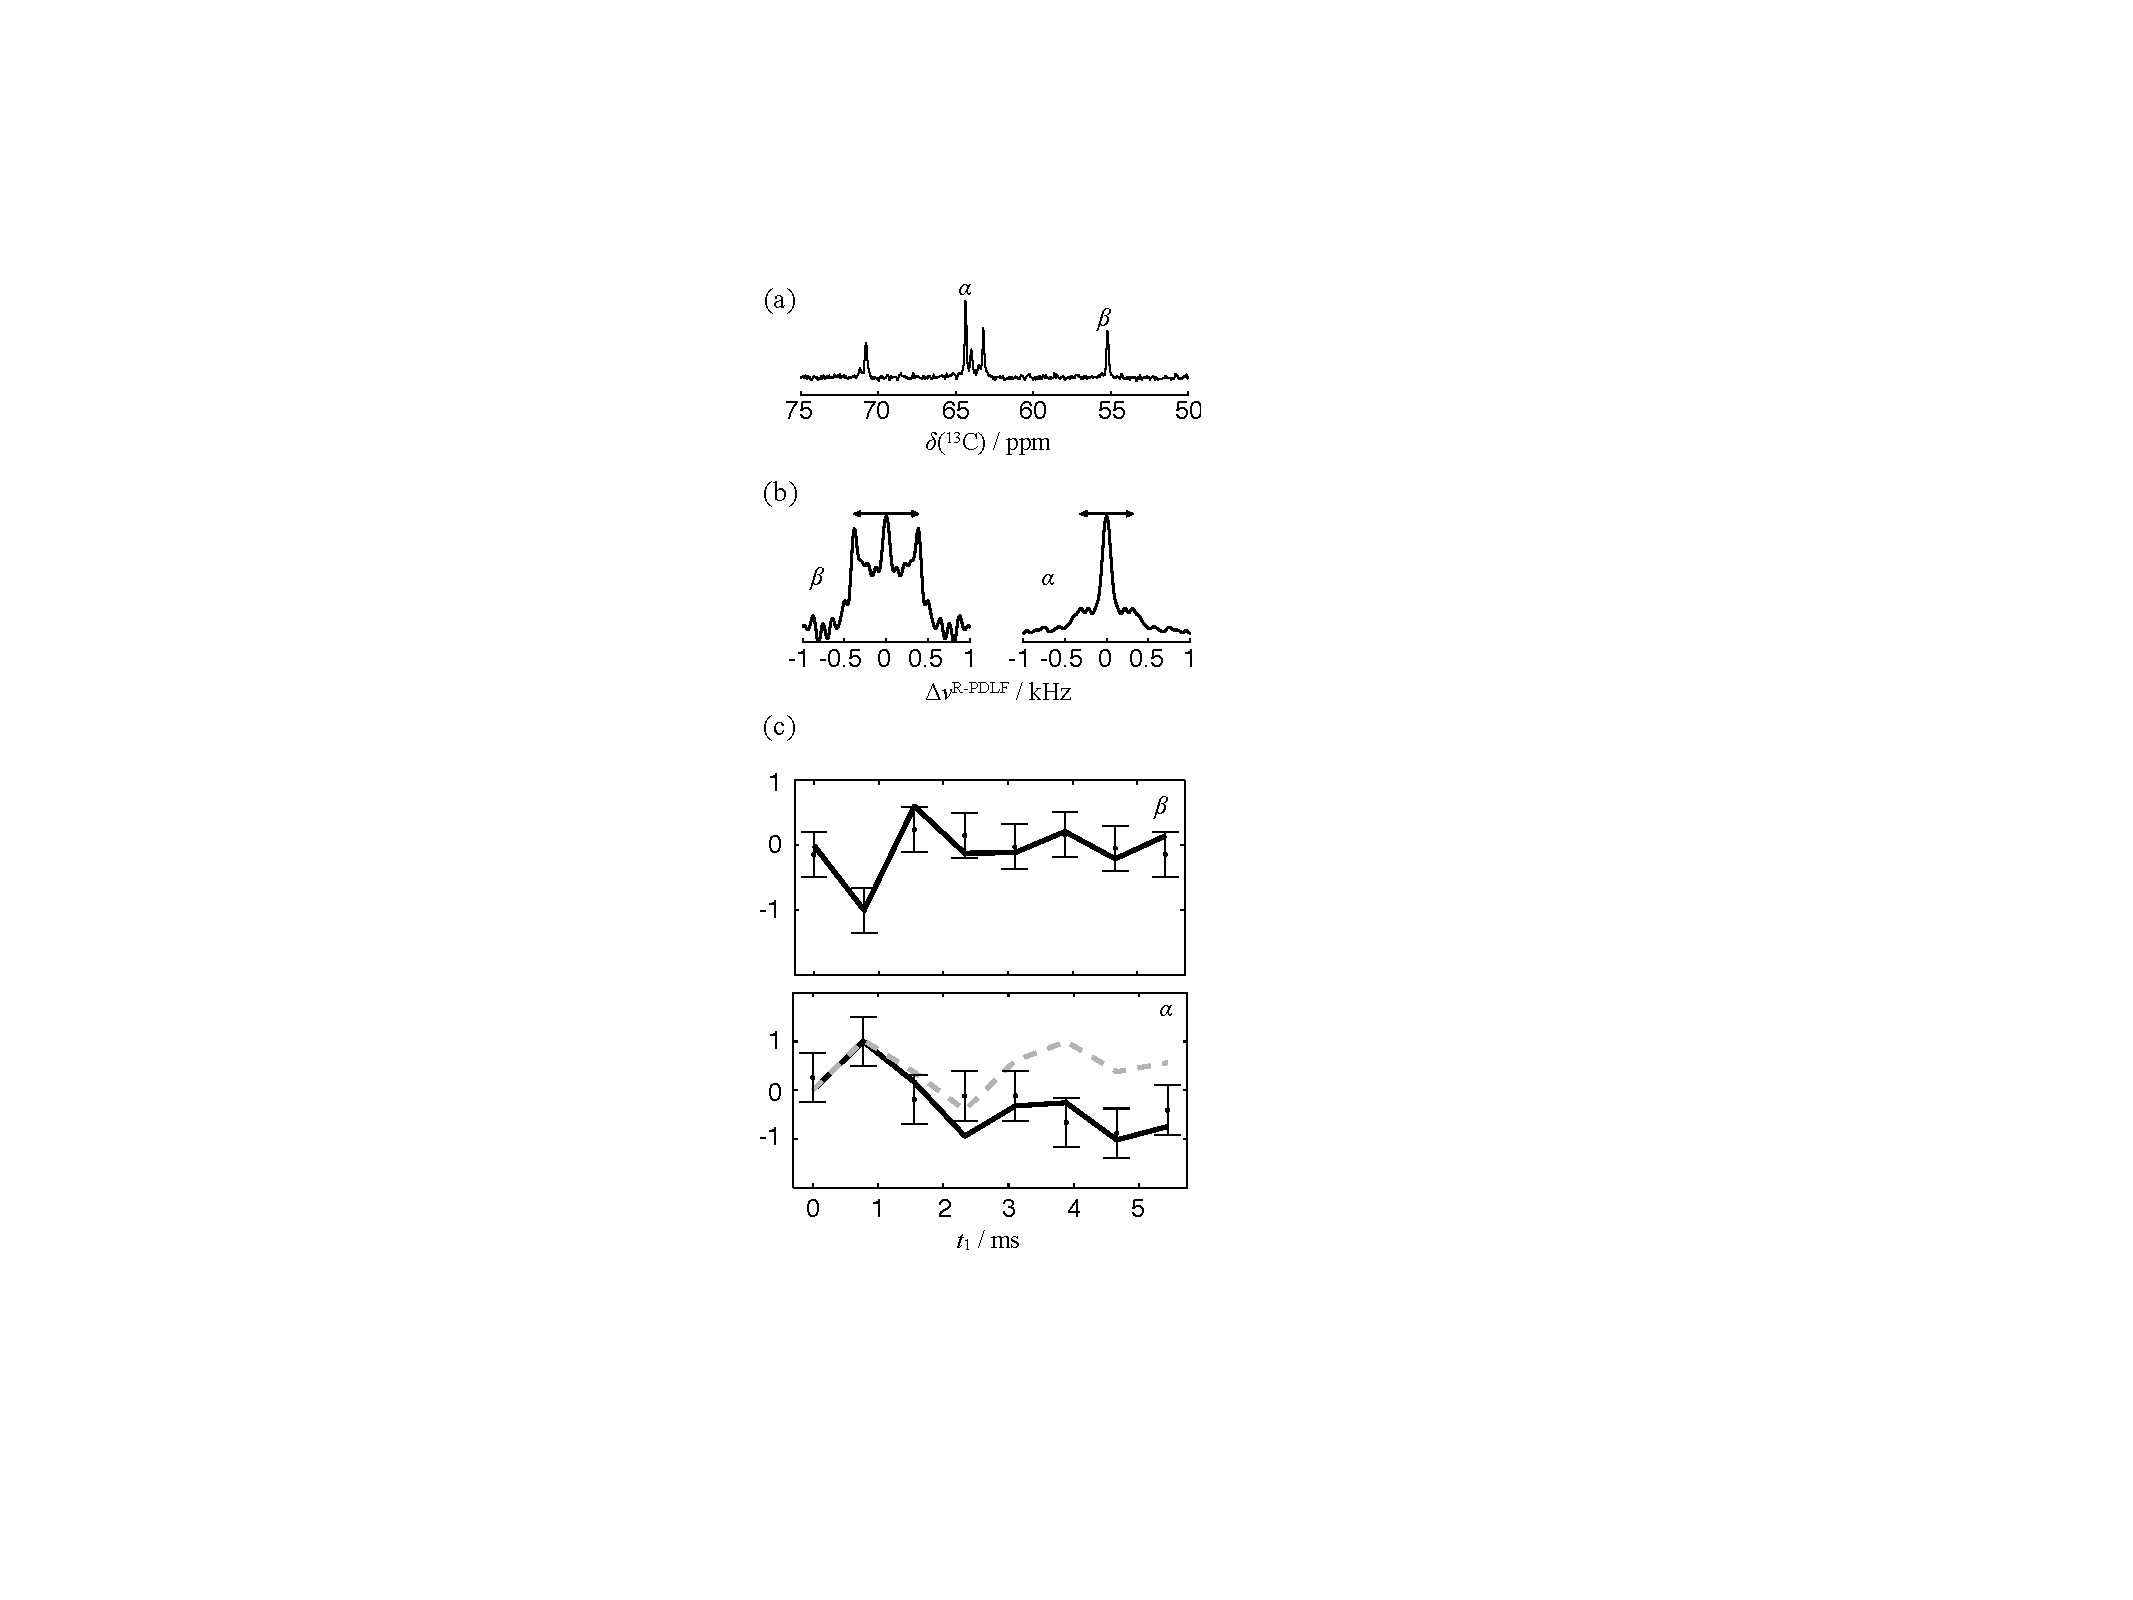
\includegraphics[width=6.0cm]{../Figs/PShgSIGNSsimpson.pdf}
  \caption{\label{PShgSIGNSsimpson}
    (a) The headgroup region of the INEPT spectrum where alpha and beta are
    identified.
    (b) The R-PDLF slices for alpha and beta showing one single
    splitting for beta (which gives an order parameter equal to 0.12), and for alpha a superposition
    of a large splitting (order parameter equal to 0.09) and a very small splitting which cannot
    resolved with the available resolution.
    (c) Points with error bars are the experimental SDROSS data.
    The thick lines are SIMPSON simulations.
    The S-DROSS slice for beta clearly shows that the order parameter is negative,
    which is confirmed by SIMPSON simulations using the order parameter value of -0.12.
    The S-DROSS slice for alpha suggests that the higher order parameter is positive
    and the deviation towards negative values in the longer t1 times suggests
    that the smaller order parameter is negative.
    This is confirmed by SIMPSON simulation using value of 0.09
    for the larger alpha order parameter and the value of -0.02 for
    smaller (black curve). The value for the smaller
    alpha order parameter for SIMPSON calculation was taken from Fig 3 in Ref. \citenum{roux91},
    because resolution in 13C NMR experiments was nor high enough to determine
    numerical value for this. The S-DROSS curve from SIMPSON simulation with positive value
    for the smaller order parameter gave did not agree with experiments (dashed grey),
    confirming the interpretation that the smaller order parameter is negative.
  }
  \todo{Maybe we should combine this with \ref{glycerolNMR}}
\end{figure}

\begin{figure}[!htb]
  \centering
  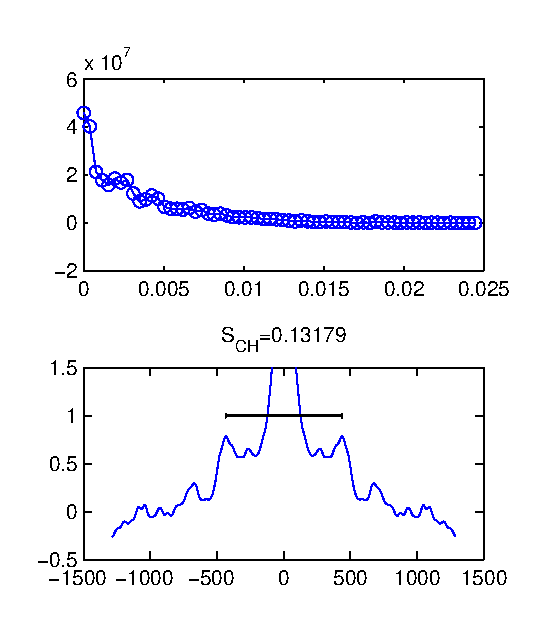
\includegraphics[width=5.5cm]{../Figs/g1_slice_large.eps}
  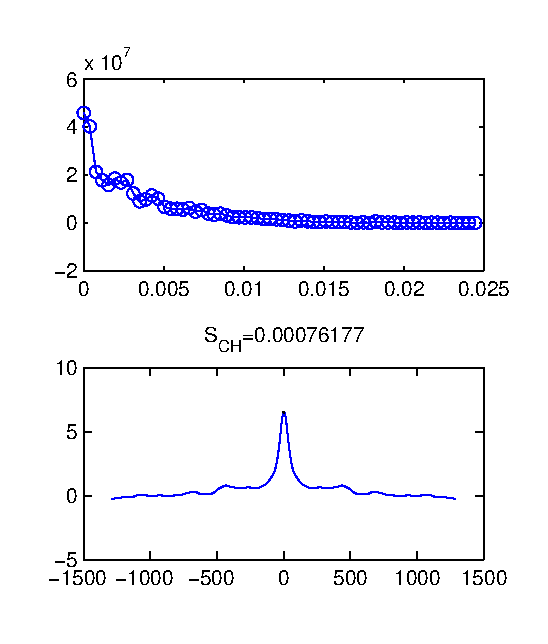
\includegraphics[width=5.5cm]{../Figs/g1_slice_small.eps}
  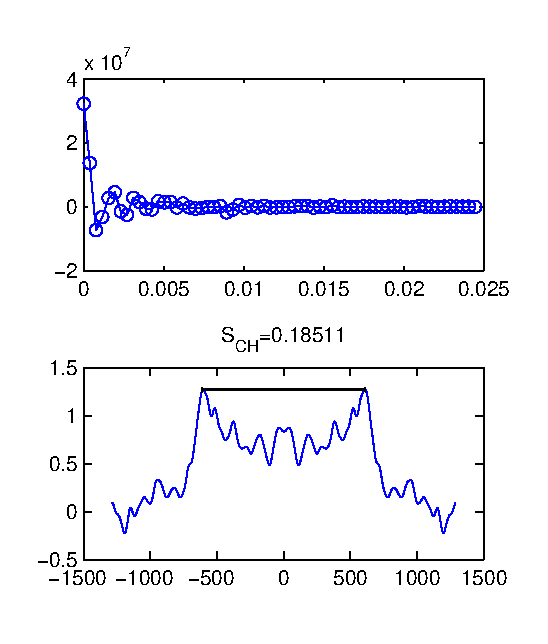
\includegraphics[width=5.5cm]{../Figs/g2_slice.eps}
  \caption{\label{glycerolNMR}
    R-PDFL slices for gycerol backbone carbons.
  }
  \todo{We need nicer figure for this data. Maybe combine with \ref{PShgSIGNSsimpson}} \\
  \todo{What are the top figures actually?}
\end{figure}

The headgroup and glycerol backbone order parameters of 
POPS measured in this work are compared to the literature values of
DOPS \cite{browning80} and POPC \cite{ferreira13} in Fig. \ref{HGorderParameters}. 
Our results for POPS are in good agreement with the previously reported
values for DOPS measured with $^2$H NMR. Significant differences are
observed between PC and PS lipids, especially at the headgroup region.  
Previous discussions in the literature have concluded that  
glycerol backbone structure is largely similar in
PC, PE, PG and PS lipids \cite{gally81}. The headgroup region was
found to be similar in PC, PE and PG lipid (assuming that the signs of PE and PG
order parameters are the same as in PC), while the PS headgroup was suggested
to be more rigid \cite{wohlgemuth80,buldt81}. 
The detailed structural differences between the headgroups is, however, not known.
\begin{figure}[]
  \centering
  \includegraphics[width=9.0cm]{../Figs/HGorderparametersPCPS.eps}
  \caption{\label{HGorderParameters}
    Headgroup and glycerol backbone order parameters of POPS measured in this work compared
    with values for DOPS ($^2$H NMR, 0.1M of NaCl) \cite{browning80} and 
    POPC  ($^{13}$C NMR) \cite{ferreira13} from literature. Signs for PS order parameters
    as measured in this work and signs for PC as measured in Refs \cite{??,ferreira16}.
    %POPG from \cite{borle85} contains 10nM PIPES, DPPG from \cite{wohlgemuth80} contains  10mM PIPES and 100mM NaCl,
    %DPPE from \cite{seelig76}, E.coliPE and E.coliPG are from \cite{gally81}.
  }
\end{figure}


%\begin{figure}[]
%  \centering
%  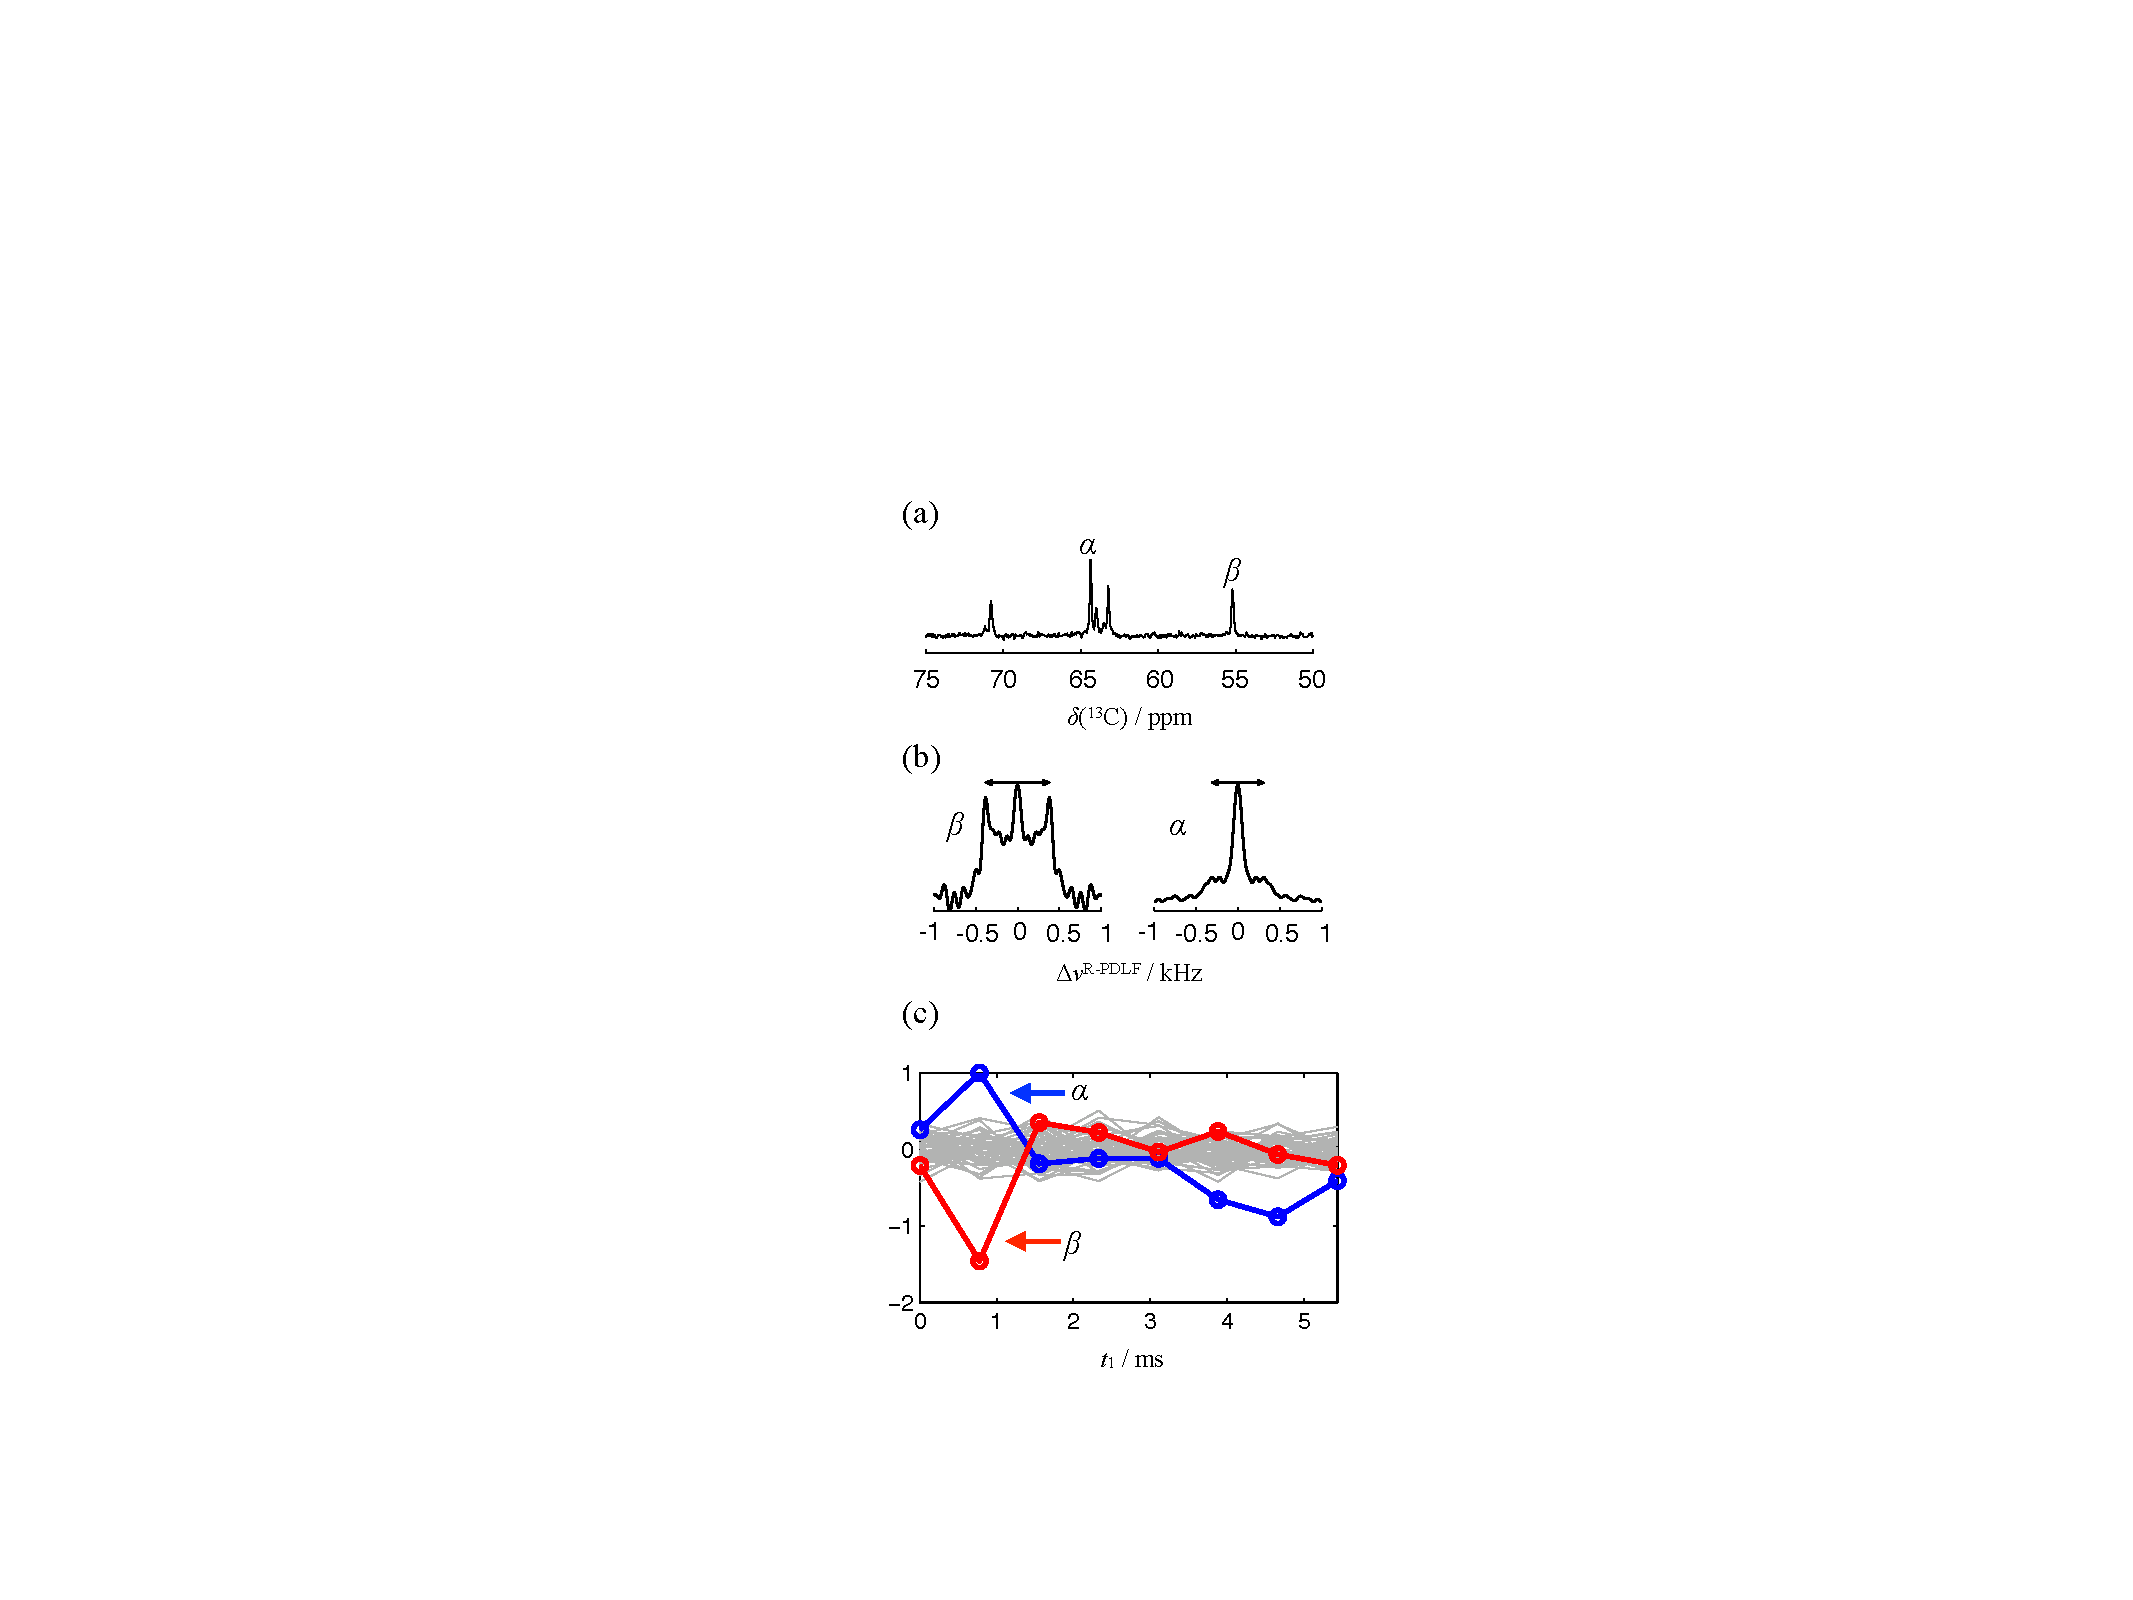
\includegraphics[width=9.0cm]{../Figs/PShgSIGNS.pdf}
%  \caption{\label{PShgSIGNS}
%    Experimental results for sign measurement for POPS sample
%  }
%\end{figure}


\subsection{Headgroup and glycerol backbone in simulations of PS lipid bilayers without additional ions}
\begin{figure}[]
  \centering
  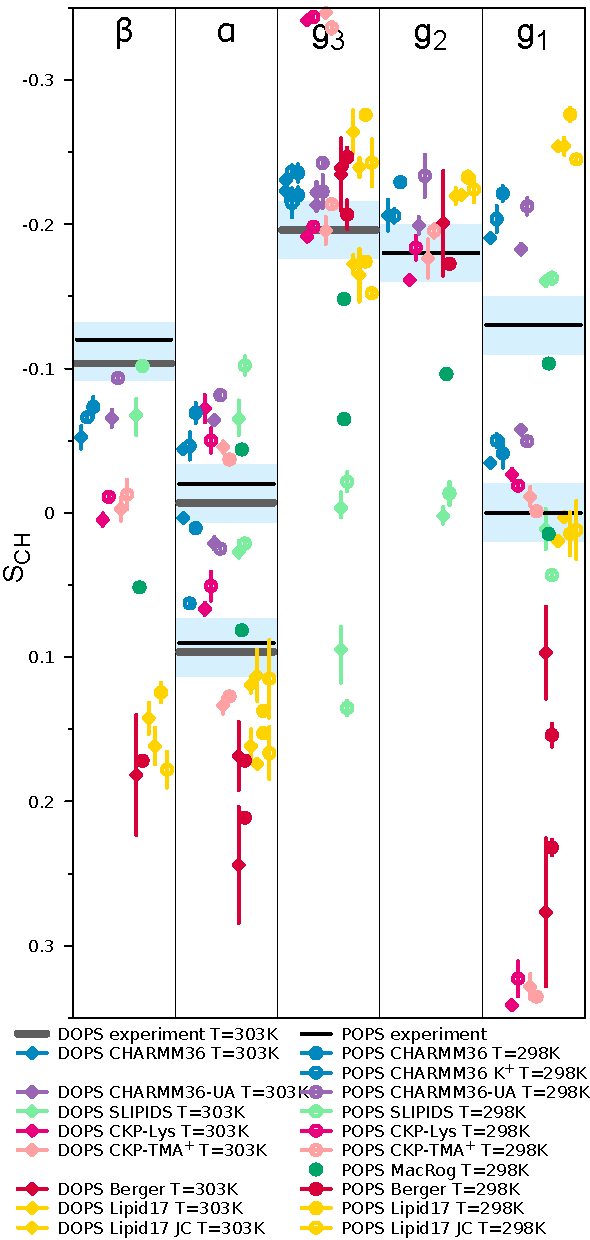
\includegraphics[width=9.0cm]{../Figs/HGorderparametersPS.pdf}
  \caption{\label{HGorderParametersPS}
    Order parameters for PS headgroup and glycerol
    backbone from simulations with different models and experiments without CaCl$_2$ 
    Experimental data from \cite{browning80} contains 0.1M of NaCl.
    Signs are taken from experiments for POPS described in Supplementary Information.
    The vertical bars shown for the computational values are not error bars, but demonstrate that for these systems we had at least two data sets; the ends of the bars mark the extreme values from the sets, and the dot marks their measurement-time-weighted average.
  }
  \todo{CHARMM36-UA point for alpha in wrong place?} \\
  \todo{MacRog POPS data should be added.} \\
  \todo{In table \ref{IONsystems}: ''CKP1 referes to the version with  
    Berger/chiu NH3 charges compatible with Berger
    and CKP2 to the version with more Gromos compatible version.'' Is this correct
    also in this figure?} \\
  \todo{Lipid17 results should be added.} \\
  \todo{We should also add CHARMM36 POPS ran with K counterions: https://github.com/NMRLipids/NMRlipidsIVotherHGs/issues/1\#issuecomment-308570874}
\end{figure}

\begin{figure}[]
  \centering
  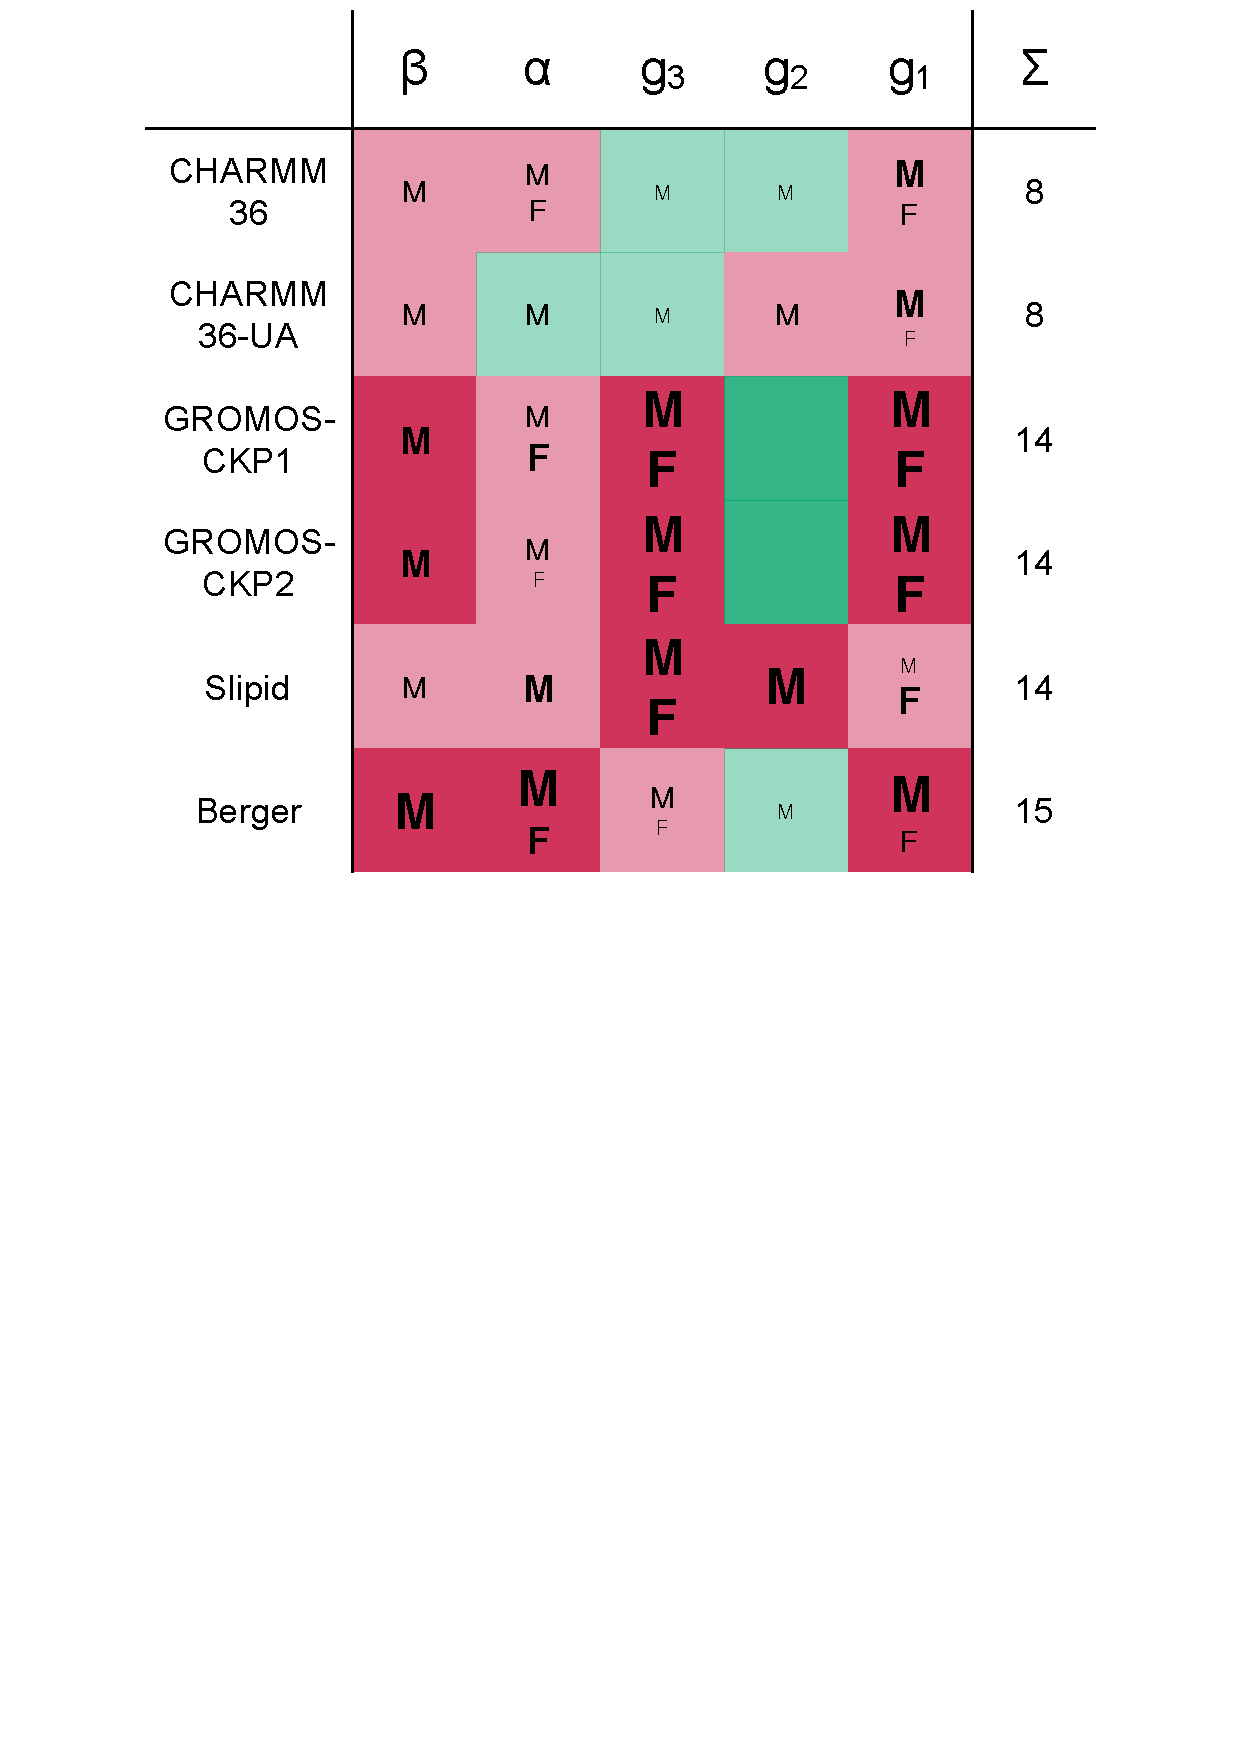
\includegraphics[width=9.0cm]{../Figs/comparisonTablePS.pdf}
  \caption{\label{comparisonTablePS}
  Rough subjective ranking of force fields based on Figure~\ref{HGorderParametersPS}. Here ÒMÓ indicates a magnitude problem, ÒFÓ a forking problem; letter size increases with problem severity. Color scheme: Òwithin experimental errorÓ (dark green), Òalmost within experimental errorÓ (light green), Òclear deviation from experimentsÓ (light red), and Òmajor deviation from experimentsÓ (dark red). The $\Sigma$-column shows the total deviation of the force field, when individual carbons are given weights of 0 (matches experiment), 1, 2, and 4 (major deviation). For full details of the assessment, see Supplementary Information.
  }
  \todo{Issue about possible updates to this plot: https://github.com/NMRLipids/NMRlipidsIVotherHGs/issues/4}
\end{figure}

The headgroup order parameters of DOPS and POPS bilayers 
from different simulation models are compared with the experimental
data in Fig. \ref{HGorderParametersPS}. In line with the previous
study for PC lipids \cite{botan15}, the glycerol backbone order 
parameters in CHARMM36 roughly agree with the experimental data,
while significant discrepancies for glycerol backbone carbons
are observed in other models.
\todo{Discussion to be finished once all the results are in the plot.}

Based on the subjective ranking shown in Fig. \ref{comparisonTablePS},
the CHARMM36 is the best performing model for both lipids.
However, none of the tested models give a satisfactory 
agreement with experiments for the headgroup order paramaters of 
PS lipids. The total deviation from the experiments ($\Sigma$ in Fig. \ref{comparisonTablePS})
for the best performing CHARMM36 model is larger for PS lipids (8)
than for PC (3) \cite{botan15}. Therefore the 
interpretation of structural details of PS headgroup or
differences between PC and PS lipids is very challenging 
from the current MD simulation models.
Figures \ref{dihedralsGLY} and \ref{dihedralsHG} show dihedral
angle distributions calculated from different models. 
The glycerol backbone structures from CHARMM36 and
Slipids simulations visualized in Fig. \ref{glycerol_buslaev} reveal the
missing structures in Slipids model, which probably lead to the incorrect
order parameters. For the headgroup $\alpha$ and $\beta$ carbon order parameters of PS lipids,
the tested models perform less well than for PC headgroup in previous
study \cite{botan15}.
\todo{Discussion will be finished when we have all the data in
  Figs. \ref{HGorderParametersPS}, \ref{dihedralsGLY} and \ref{dihedralsHG}}

\begin{figure}[]
  \centering
  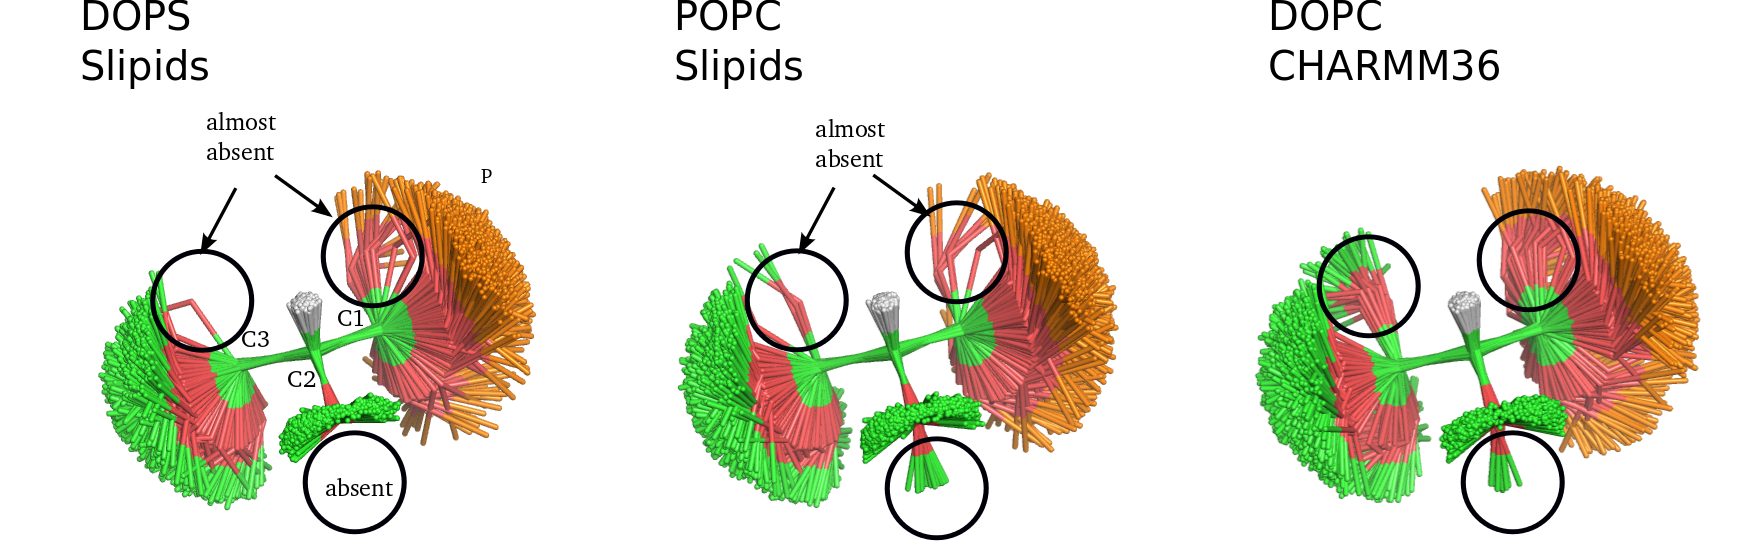
\includegraphics[width=9.0cm]{../Figs/glycerol_buslaev.png}
  \caption{\label{glycerol_buslaev}
    Snapshots overlayed from different simulations for glycerol backbone region
    by Pavel Buslaev.
  }
\end{figure}

Since systems with negatively charged PS lipids always contain counterions
and the ion binding presumably affects the PS headgroup
order parameters, the discussion of ion binding affinity and
headgroup structure cannot be separated as done previously
for PC lipids \cite{botan15,catte16}. The density profiles
of counterions along membrane normal from different simulations
are shown in Fig. \ref{NAdensPOPS}.
Significant differences are observed in counterion
densities between different simulation models. 
\todo{We should try to figure out which one of these are more
  realistic. One option could be to use PS headgroup order parameter
  data measured as a function of NaCl \cite{roux86}. Another
  approach could be to use the area per molecule, which is suggested to
  depend on the binding affinity of counterions \cite{pandit02,mukhopadhyay04,pedersen06}. The
  experimental value for area per molecule is available at \cite{pan14}.}
\begin{figure}[]
  \centering
  \includegraphics[width=9.0cm]{../Figs/NAdensPOPS.eps}
  \caption{\label{NAdensPOPS}
    Counterion densities of POPS lipid bilayer along the membrane normal from
    simulations with different force fields.
  }
\end{figure}

\subsection{Headgroup structure in PS and PC mixtures}
Lipid mixtures containing PC and PS lipids are present in biological
systems. Also the Ca2+ binding affinity to bilayers containing
PS lipids is measured from mixtures with PC, because pure PS
bilayers exhibit instant transition to the ordered phase with the
addition of the ions. Therefore, the characterization of mutual interactions
between PC and PS lipid headgroups is necessary in order to
understand PS lipids in biological environments.

Fig. \ref{HGorderparametersPCvsPS} shows the headgroup order parameters
of POPC and POPS lipids in mixtures with various mole fractions from 
simulations and experiments \cite{scherer87,roux90}.
The headgroup order parameters of POPC increase with the increasing
amount of negatively charged POPS, as expected from the 
the electrometer concept \cite{seelig87}. Notably, the concept
seems to be generally valid, at least qualitatively, also for 
other lipid mixed with PC lipids; the PC lipid headgroup order
parameters increase when mixed with negatively charged 
lipids (PS, PI, CL, PA and PG) and remains almost unchaged when 
mixed with neutral lipids (PE and SM) \cite{scherer87} or cholesterol \cite{ferreira13}.
This is, however, not reproduced in the simulation data 
in Fig. \ref{HGorderparametersPCvsPS}. The order parameter for
$\beta$-carbon of POPC decreases and almost negligible increase is 
seen in $\alpha$ order parameter with the addition of PS lipid in CHARMM36 simulation.
This may indicate incorrect interactions between PC and PS headgroups
in simulations. On the other hand, the previously reported overestimated
ion binding affinity may also play a role, as the amount of counterions
is increasing with PS.
\todo{Data from other force fields to be collected before discussion can be finalized.}

\begin{figure*}[]
  \centering
  \includegraphics[width=16.0cm]{../Figs/HGorderparametersPCvsPS.eps}
  \caption{\label{HGorderparametersPCvsPS}
    Headgroup order parameters from PC:PS mixtures from 
    different simulation models and experiments.
    Left panel shows the PC headgroup order parameters (experimental results from Ref. \citenum{scherer87},
    signs are determined as discussed in \cite{botan15,ollila16}).
    Rigth panel shows PS headgroup order parameters (experimental result for pure POPS measured in this
    work at 298K, experimental result for mixture from Ref. \citenum{roux90} at 298K).
    Counterions in expriments are sodium, while potassium is used in simulations.
    Using sodium in simulations do not have a significant effect.
  }
  \todo{Simulation of CHARMM36 at 298K should be maybe rerun with Gromacs 5.} \\
  \todo{We need results also from other than CHARMM36 force field.}
\end{figure*}

Also the headgroup order parameters of POPS mixed with varying amounts of POPC
from simulations and experiments \cite{borle85,roux90} are shown in Fig. \ref{HGorderparametersPCvsPS}.
The $\beta$-carbon order parameter of POPS slightly decreases and positive 
order parameter of $\alpha$-carbon slightly increases with increasing
amount of PS lipids. This may indicate increasing order of the headgroup.
It should be, however, noted that the experimental data for pure POPS and
POPC/POPS mixture come from different experimental sets, 13C NMR in this work
and 2H NMR from Ref. \citenum{roux90}, respectively. Therefore the accuracy
of the order parameter change is not as high as typically in the measurements
of order parameter changes, see discussion about qualitative and quantitative 
accuracy in Ref. \citenum{ollila16}. The changes of PS headgroup order parameters
are not reproduced by the tested simulation models. The $\beta$-carbon order parameter
increase with increasing amount of PS in CHARMM36 and MacRog simulations in contrast
to the experimental data. The smaller $\alpha$-carbon order parameter increase in both
simulation models with increasing amount of PS, while it is almost unchanged in experiments.
The larger $\alpha$-carbon order parameter increase in MacRog and decrease in CHARMM36
with increasing amount of PS, both model exhibiting a poor agreement with experiments. 
Signifincant improvement in the MD simulation models are needed to interpret the
PS headgroup structures and mutual interactions with PC lipids. 

\subsection{Ca$^{2+}$ binding affinity in bilayers with negatively charged PS lipids}

The headgroup order parameters of PC lipids can be used to measure ion binding
affinity because they change proportionally
to the amount of bound charge in bilayer \cite{seelig87,catte16}.
This molecular electrometer concept can be applied also to
lipid bilayers with mixtures of PC and negatively charged
lipids \cite{borle85,macdonald87,roux90}.
This is demonstrated in Fig. %s \ref{OrderParametersWithCaCl},
%\ref{OrderParametersWithCaClBELOW1M} and
\ref{OrderParameterCHANGESWithCaClBELOW1M}
using the previuosly reported experimental data
for mixtures with varying proportions of
negatively charged PS or PG lipids.
%
%the changes of PC headgroup order parameters %for PC headgroup $\alpha$ and $\beta$ carbons
%as a function of CaCl$_2$ concentration are shown
%
As expected, the decrease of order parameters with CaCl$_2$
is more pronounced for systems with more
negatively charged lipids.
% (see Fig. \ref{OrderParameterCHANGESWithCaClBELOW1M}).



%PC headgroup order parameters increase when negatively charged
%PS or PG are added to PC bilayer in the absense of added CaCl$_2$,
%as expected based on electrometer concept \cite{seelig87}
%(see Fig. \ref{OrderParametersWithCaClBELOW1M}).
%In electrometer concept this is explained by the tilting of
%headgroup more parallel to membrane normal \cite{??}.

%Order parameters reach the values of pure PC bilayer close to CaCl$_2$ concentrations of $\sim$ 50-300mM.
%At this point the Ca2+ binding presumably fully cancels the charge from negative lipids and
%overcharging occurs above these concenterations.


Before using the headgroup order parameters to compare ion binding affinity between simulations
and experiments, it is important to quantify the response of the order parameters to the
bound charge in simulations.
The response of headgroup order parameters to the fixed amount of cationic surfactants in
POPC bilayer is compared between simulations and experiments \cite{scherer89} In Fig. \ref{CHANGESwithCaClPGPS}.
The figure shows that the order parameters are too sensitive to bound charge in Lipid14 model,
while CHARMM36 is in better agreement with experiments. This has to be taken into account when
analysin the binding affinities.
\begin{figure}[]
  \centering
  \includegraphics[width=9.0cm]{../Figs/HGopsDHMDMAB.eps}
  \caption{\label{CHANGESwithCaClPGPS}
  The response of headgroup order parameters to the fixed amount of cationic surfactants in
  POPC bilayer is compared between simulations and experiments \cite{scherer89}.}
\end{figure}

The headgroup order parameter changes of POPC and POPS from POPC:POPS (5:1) bilayers
as a function of Ca$2+$ concentration from different
simulations and experiments \cite{roux90} are shown in Fig. \ref{changesWITHCaClPG}.
As shown previously, the changes of PC headgroup order parameters can be
used to measure the amount of bound ions to the bilayer according to the
electrometer concept \cite{akutsu81,seelig87,catte16}.
This would suggest that the Ca2+ binding is overestimated in
MacRog simulation and underestimated in CHARMM36 simulation.
It should be however noted, that MacRog simulation with low
concentrations gives a good agreemet with experiments.
The result from CHARMM simulation is somewhat surprising because
previous study suggested that Ca2+ ions overbind to pure PC lipid
bilayers \cite{catte16}.
\todo{The role of counterions and equilibration should be somehow checked
  and discussed.}
The density profiles of Ca2+ from the simulations are shown in Fig. \ref{CAdensPCPSmixture}.
Overall, it seems that calcium clearly overbinds in MacRog simulations
as expected based on previous results \cite{catte16}.
However, the calcium binding in CHARMM36 simulations seems to
surprisingly low. Thi
\begin{figure*}[]
  \centering
  \includegraphics[width=18cm]{../Figs/CHANGESwithCaClPS.eps}
  \caption{\label{changesWITHCaClPG}
    POPC (left) and POPS (right) headgroup order parameters in lipid bilayer with POPC:POPS (5:1) mixture
    as a function CaCl$_2$ concentration from experiments \cite{roux90} and different simulations.
  }
\end{figure*}
\begin{figure}[]
  \centering
  \includegraphics[width=9cm]{../Figs/CAdensPCPSmixture.eps}
  \caption{\label{CAdensPCPSmixture}
    Ca2+ density profiles from simulations.
  }
  \todo{Ca2+ binding in CHARMM is lower than to neutral membrane. The reason should be found out (probably equilibration).}
  \todo{These are now mass densities, numbers would be probably better.}
  \todo{Counterions should be also included.}
  \todo{Not all the data from MacRog is included.}
\end{figure}

Also dependence of $\beta$-carbon of PG on CaCl$_2$ concentration is compared with
experiments \cite{borle85} in Fig. \ref{PSPGchangesWITHCaCl}. Absolute value of
the order parameter is too large without ions, but rapid decrease due to addition of
CaCl$_2$ is observed in agreement with experiments for systems with 1:1 mixture of POPC and POPG.
In addition, absolute value in systems with CaCl$_2$ is in agreement with experiments.
However, system with 4:1 mixture of POPC and POPG behaves differently, but experimental
data is not available for comparison for this mixture.

\todo{More simulation data for systems with PS lipids and CaCl$_2$ would be probably useful}

%\subsection{Effect of Ca$2+$ binding to PS headgroup}

Also the experimental order parameters of POPS headgroup 
as a function of CaCl$_2$ concentration are shown in Fig. \ref{PSPGchangesWITHCaCl}.
The order parameter changes with added CaCl$_2$ are overestimated in
both simulation models. However, the changes can be considered qualitatively
correct for both segments in CHARMM36 model and in $\beta$ segment in MacRog model. 
\todo{These should be compared to simulations for potential structural interpretation of the changes.}
%\begin{figure}[]
%  \centering
%  \includegraphics[width=9.0cm]{../Figs/PSPGwithCaCl.eps}
%  \caption{\label{PSPGchangesWITHCaCl}
%    PG and PS order parameters a function CaCl$_2$ concentration taken from \cite{borle85} and \cite{roux90}, respectively.
%  }
%  \todo{Get the small concentration data from the inserts}
%\end{figure}





\section{Conclusions}


% Tables may be be put in the text as floats.
% Here is an example of the general form of a table:
% Fill in the caption in the braces of the \caption{} command. Put the label
% that you will use with \ref{} command in the braces of the \label{} command.
% Insert the column specifiers (l, r, c, d, etc.) in the empty braces of the
% \begin{tabular}{} command.
%
% \begin{table}
% \caption{\label{} }
% \begin{tabular}{}
% \end{tabular}
% \end{table}

% If you have acknowledgments, this puts in the proper section head.
\begin{acknowledgments}
% Put your acknowledgments here.
\end{acknowledgments}
\pagebreak
\appendix
\begin{center}
{\bf SUPPLEMENTARY INFORMATION}
\end{center}

\section{Simulated systems}


\section{PC lipid headgroup response to different mixtures in experiments}
As shown in Fig. \ref{HGorderparametersPCvsPEPSPGchol}, order parameters of PC
headgroup behave in various lipid mixtures as expected from the electrometer concept \cite{seelig87, scherer87},
i.e., order parameters increase when anionic lipids are mixed with PC and decrease with cationic
surfactants. The changes with the addition of neutral lipids is significantly smaller.
\begin{figure}[]
  \centering
  \includegraphics[width=8.0cm]{../Figs/HGorderparametersPCvsPEPSPGchol.eps}
  \caption{\label{HGorderparametersPCvsPEPSPGchol}
    PC headgroup order parameters from experiments of mixtures with
    PE, PS, PG and cholesterol \cite{scherer87,scherer89,ferreira13}.
    Signs are determined as discussed in \cite{botan15,ollila16}.
  }
\end{figure}

\section{Cation binding affinity to lipid bilayers with different amount of charge}

%\begin{figure}[]
%  \centering
%  \includegraphics[width=9.0cm]{../Figs/LIPIDSwithCaCl.eps}
%  \caption{\label{OrderParametersWithCaCl}
%    PC headgroup order parameters as a function of CaCl concentration from experiments containing charged lipids.
%    Pure DPPC data from \cite{akutsu81}, pure POPC data from \cite{altenbach84}, 
%    POPC:POPS mixture data from \cite{roux90}, POPC:POPG mixture data with 0.1M NaCl from \cite{macdonald87}
%    and POPC:POPG mixture data without NaCl from \cite{borle85}.
%  }
%  \todo{Check the NaCl concentrations in the samples.}
%\end{figure}
%\begin{figure}[]
%  \centering
%  \includegraphics[width=9.0cm]{../Figs/LIPIDSwithCaClBELOW1M.eps}
%  \caption{\label{OrderParametersWithCaClBELOW1M}
%    Figure \ref{OrderParametersWithCaCl} zoomed to smaller concentrations.
%  }
%\end{figure}
\begin{figure}[]
  \centering
  \includegraphics[width=9.0cm]{../Figs/CHANGESwithCaCl.eps}
  \caption{\label{OrderParameterCHANGESWithCaClBELOW1M}
    The change of PC headgroup order parameters
    in the presence of different amount of negatively charged lipids
    respect to the values without added CaCl$_2$.
    The original data is the same as in Fig. \ref{OrderParametersWithCaCl}. 
    Pure DPPC data from \cite{akutsu81}, pure POPC data from \cite{altenbach84}, 
    POPC:POPS mixture data from \cite{roux90}, POPC:POPG mixture data with 0.1M NaCl from \cite{macdonald87}
    and POPC:POPG mixture data without NaCl from \cite{borle85}.
  }
\end{figure}



\section{Dihedrals}
\begin{figure*}[]
  \centering
  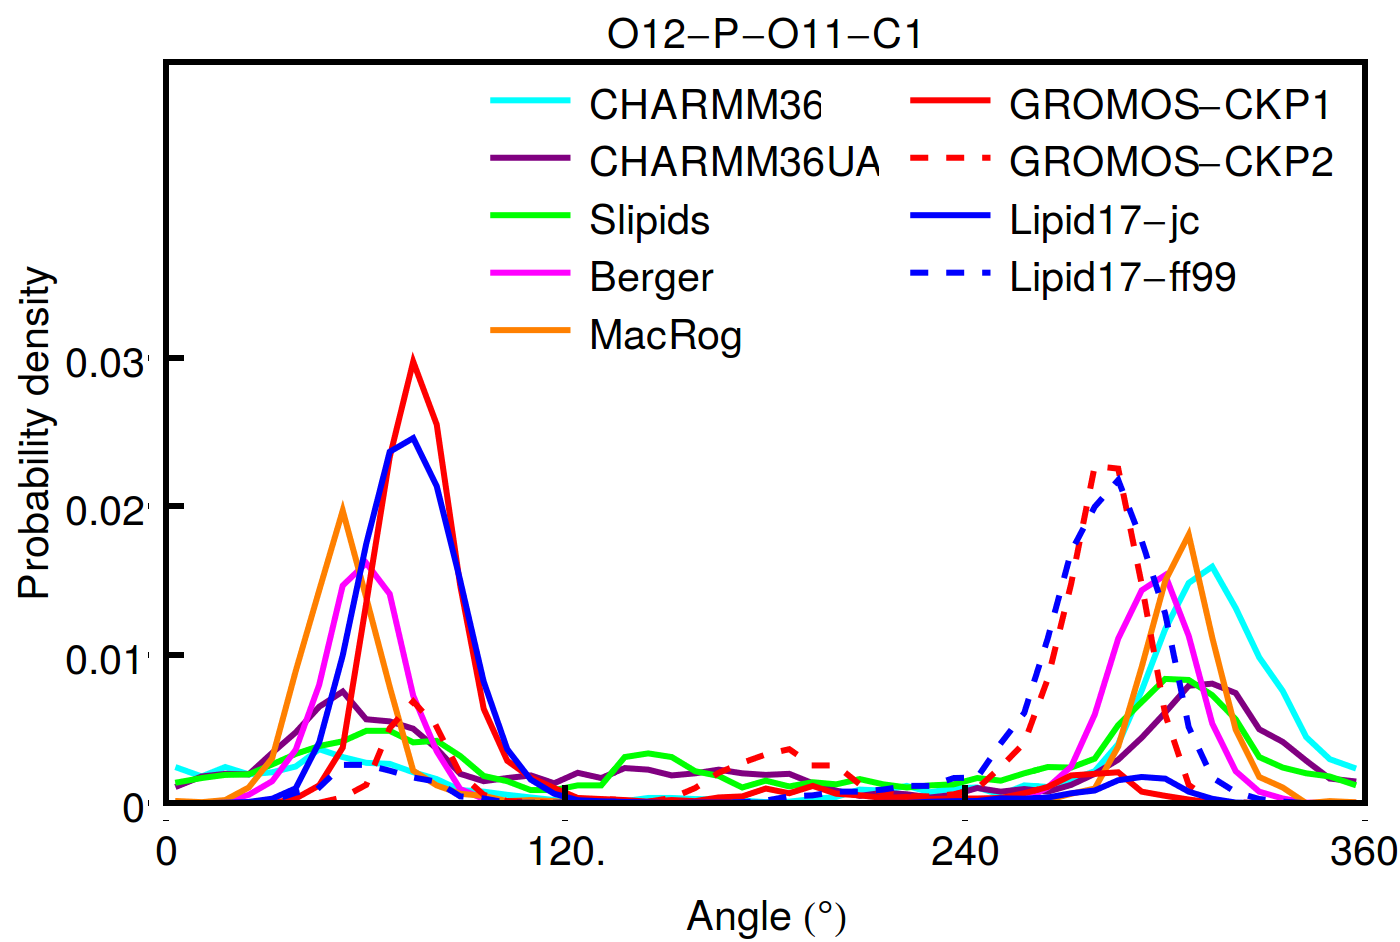
\includegraphics[width=8.0cm]{../Figs/diheds_pops1.png}
  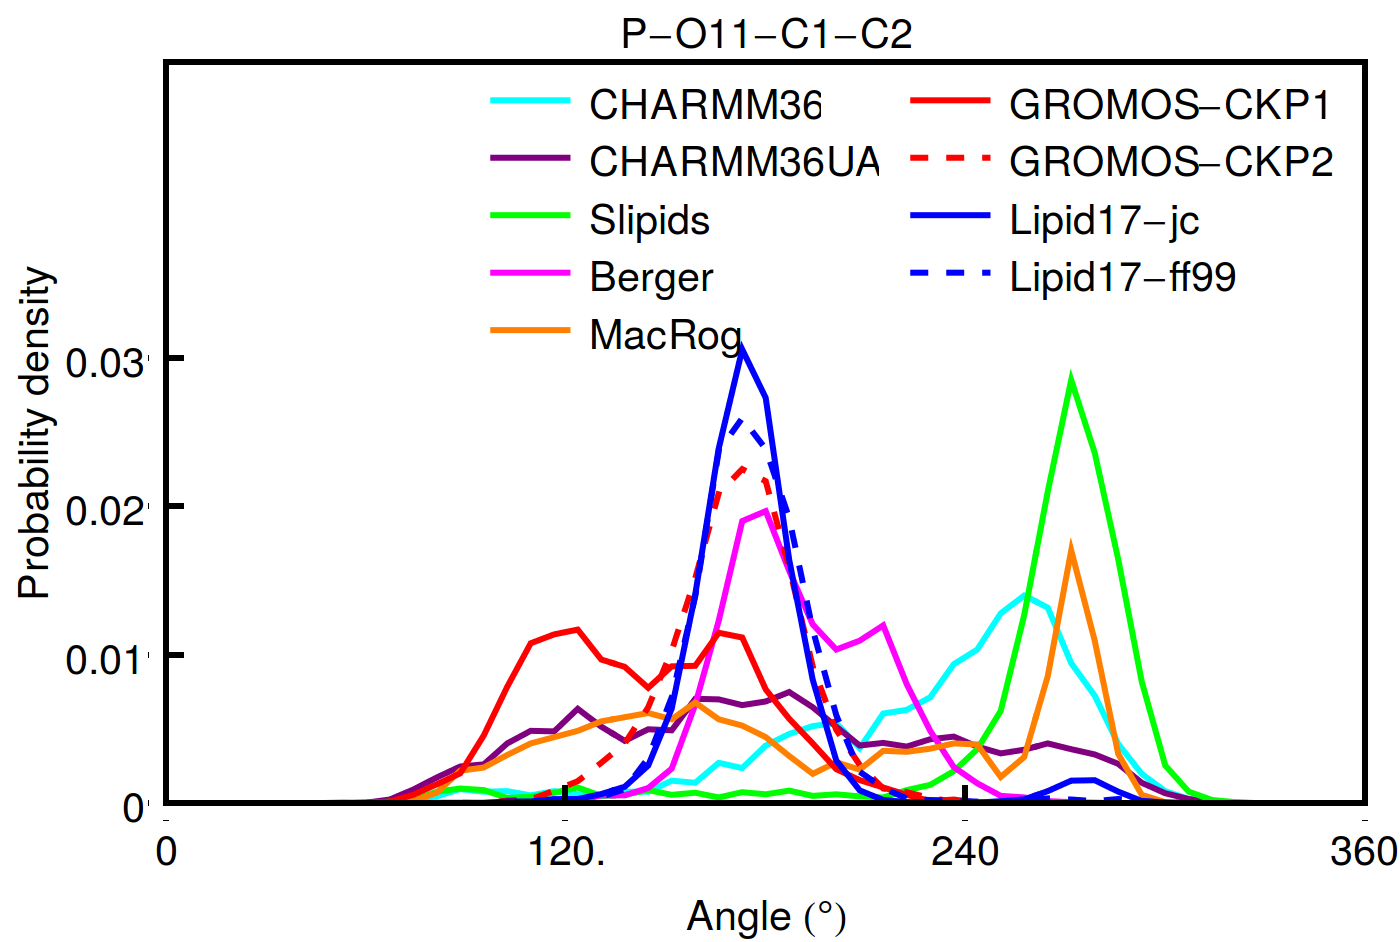
\includegraphics[width=8.0cm]{../Figs/diheds_pops2.png}
  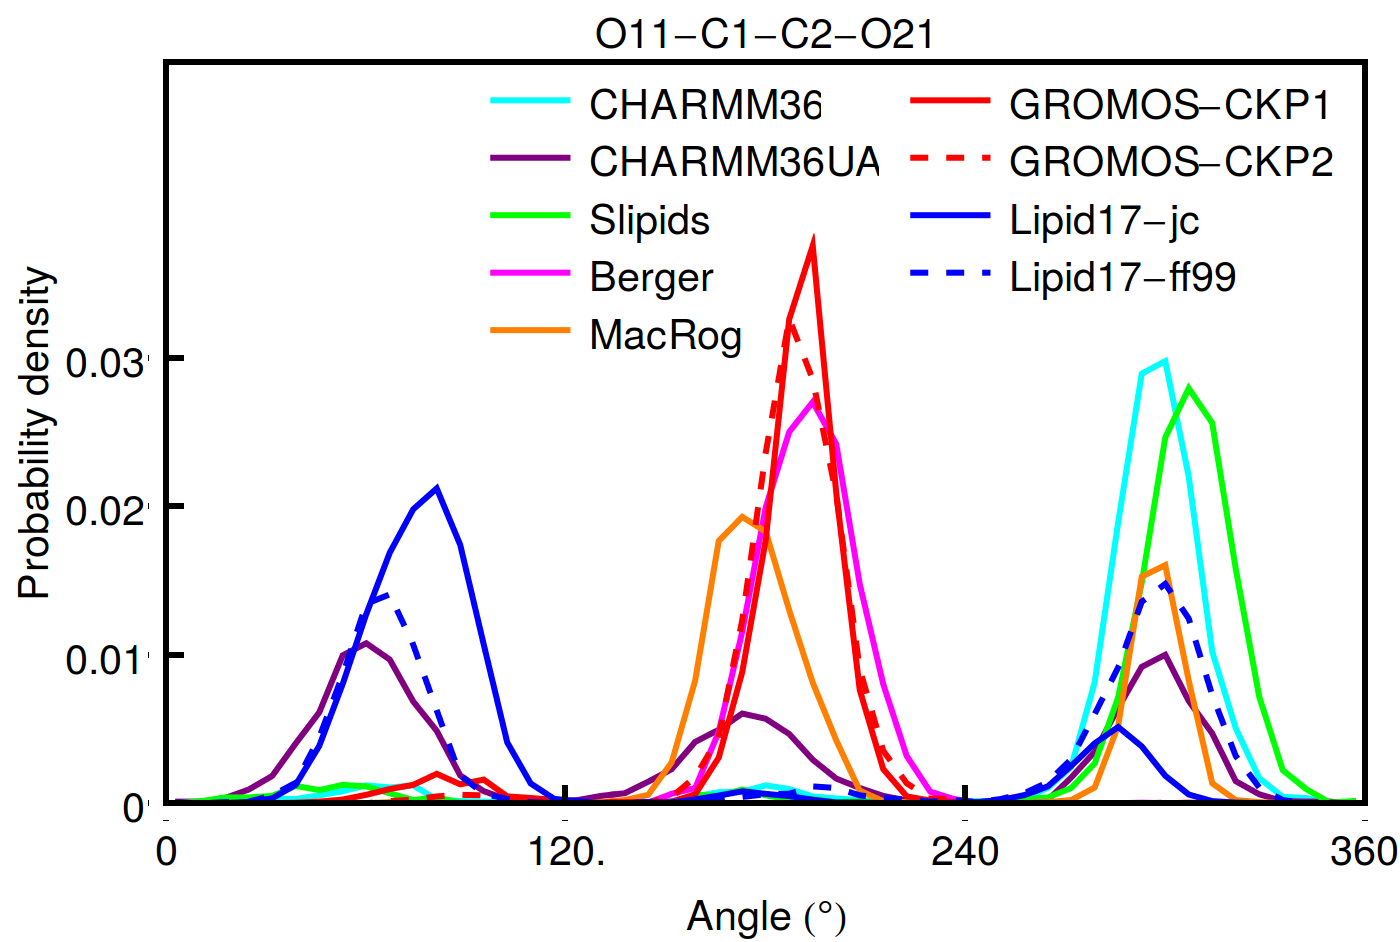
\includegraphics[width=8.0cm]{../Figs/diheds_pops3.png}
  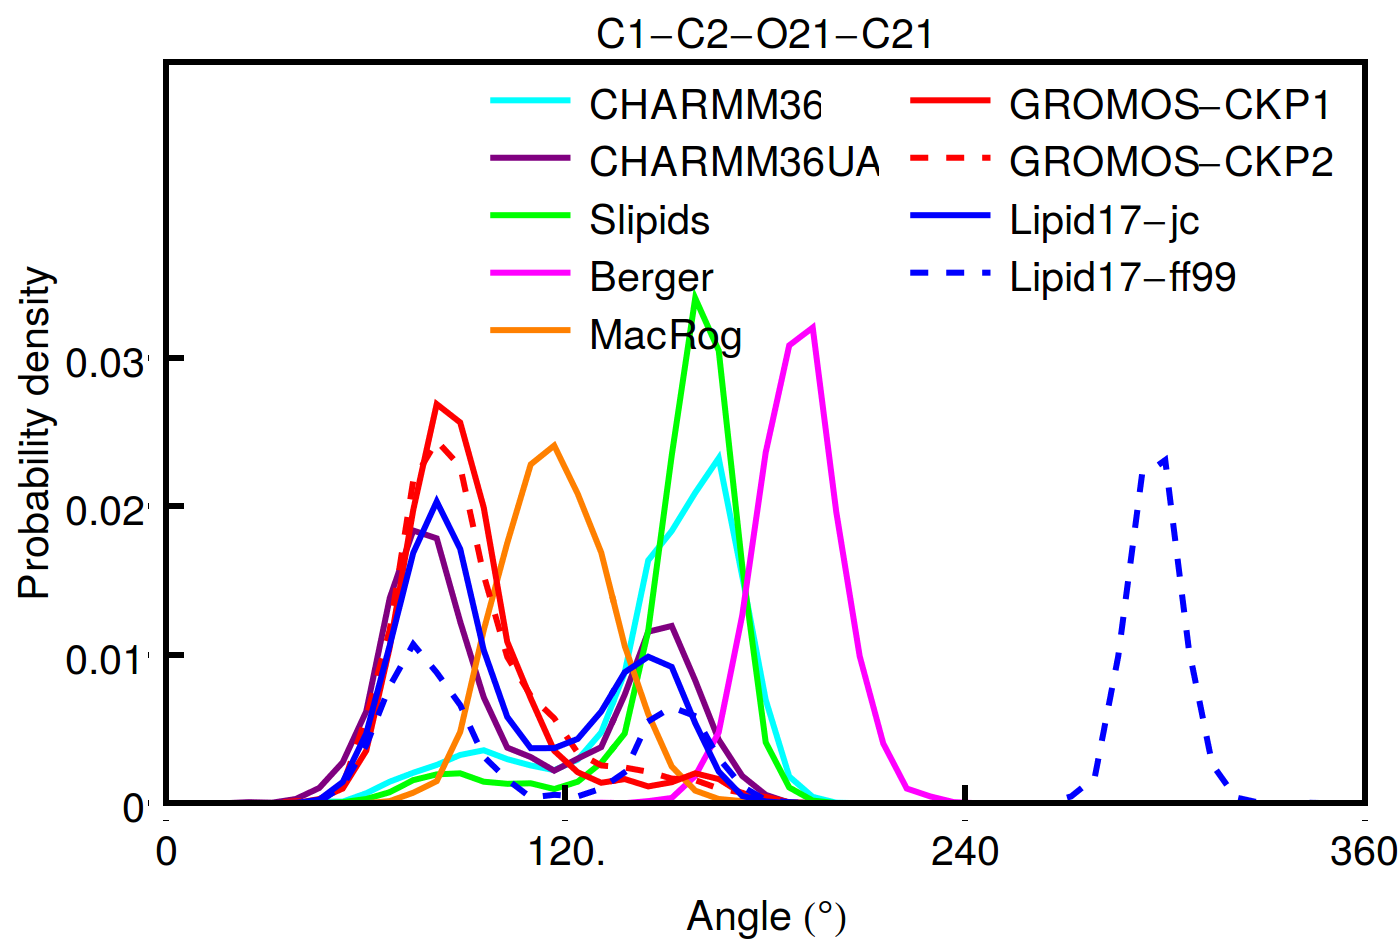
\includegraphics[width=8.0cm]{../Figs/diheds_pops4.png}
  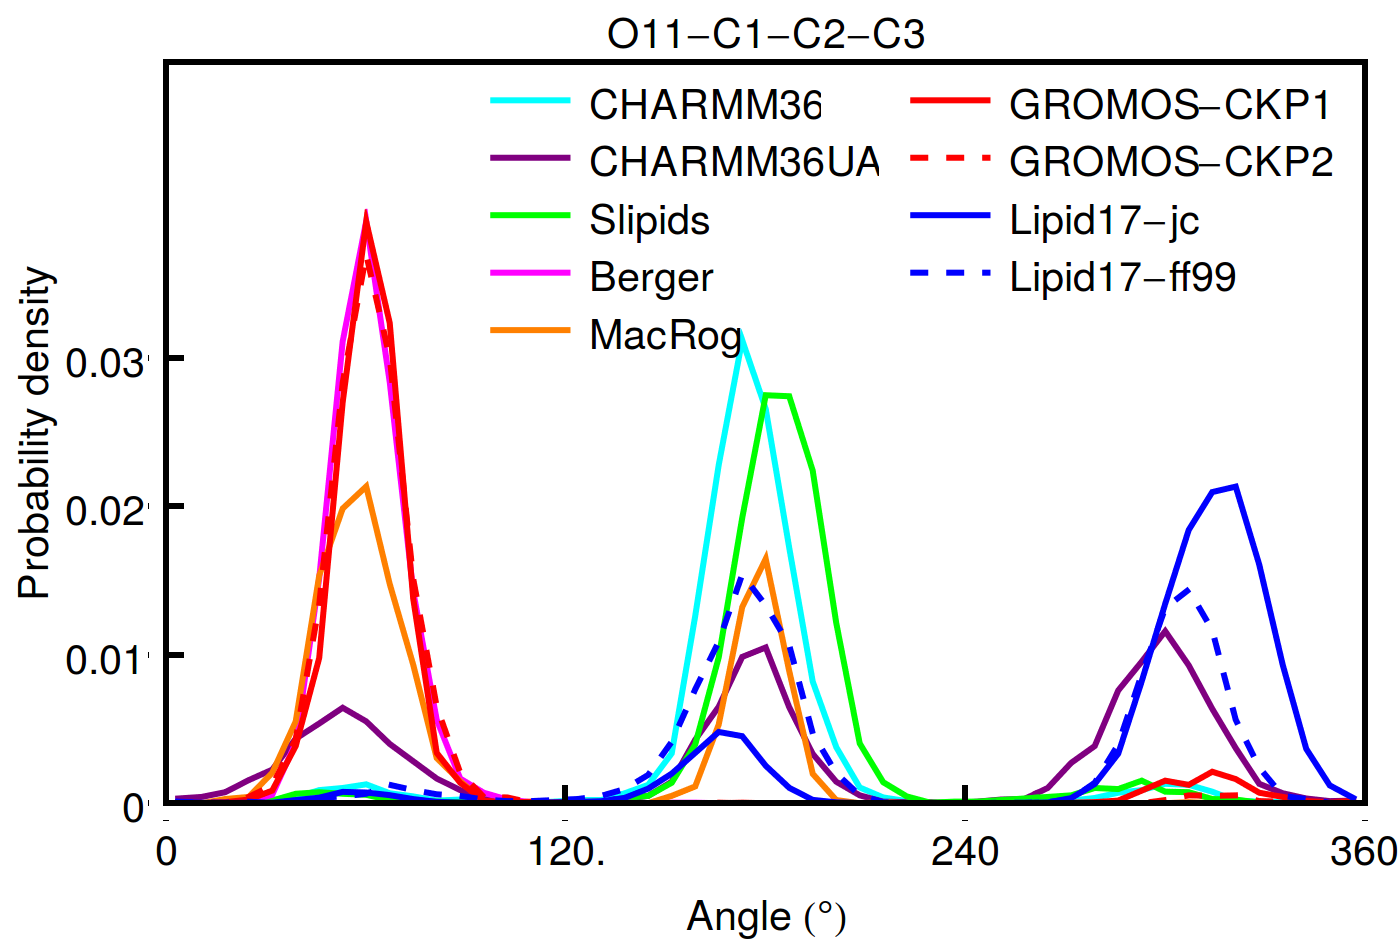
\includegraphics[width=8.0cm]{../Figs/diheds_pops5.png}
  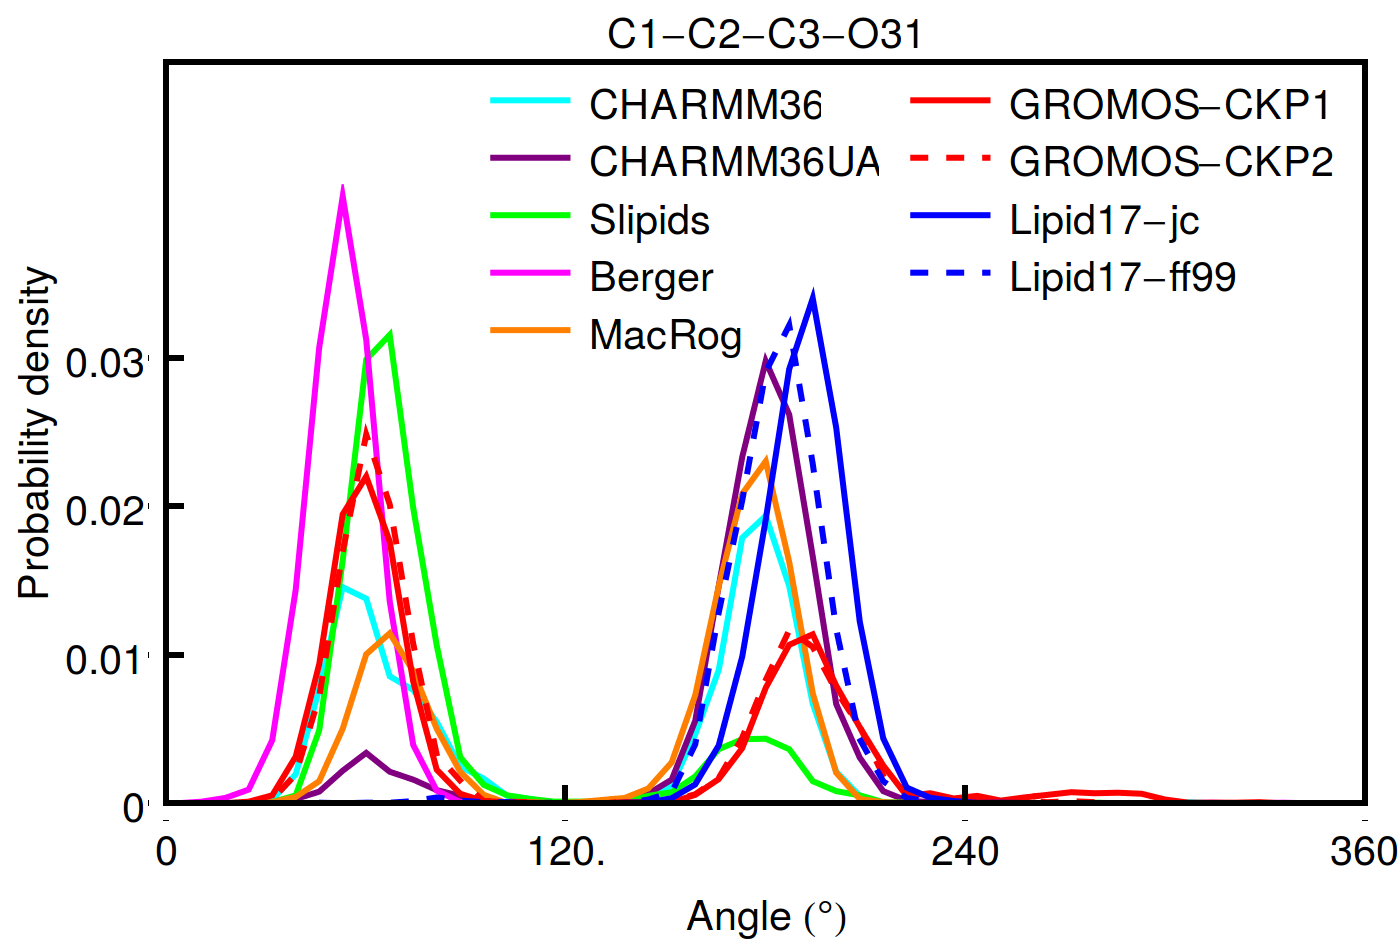
\includegraphics[width=8.0cm]{../Figs/diheds_pops6.png}
  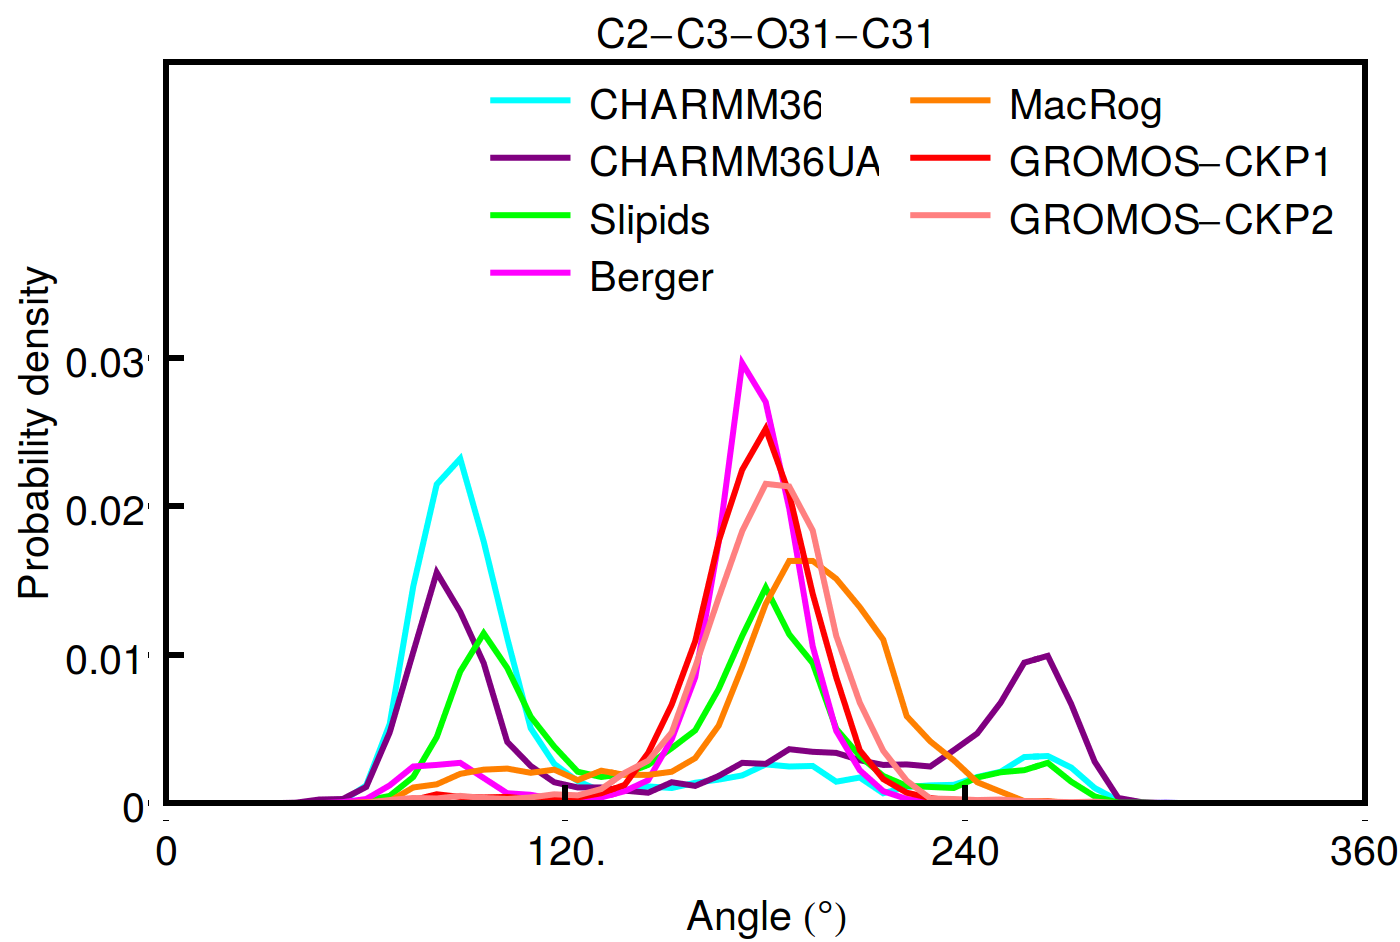
\includegraphics[width=8.0cm]{../Figs/diheds_pops7.png}
  \caption{\label{dihedralsGLY}
    Dihedral angle distributions of bonds from phosphate to acyl chain carbonyls from different simulation models.
  }
\end{figure*}
\section{Dihedrals}
\begin{figure*}[]
  \centering
  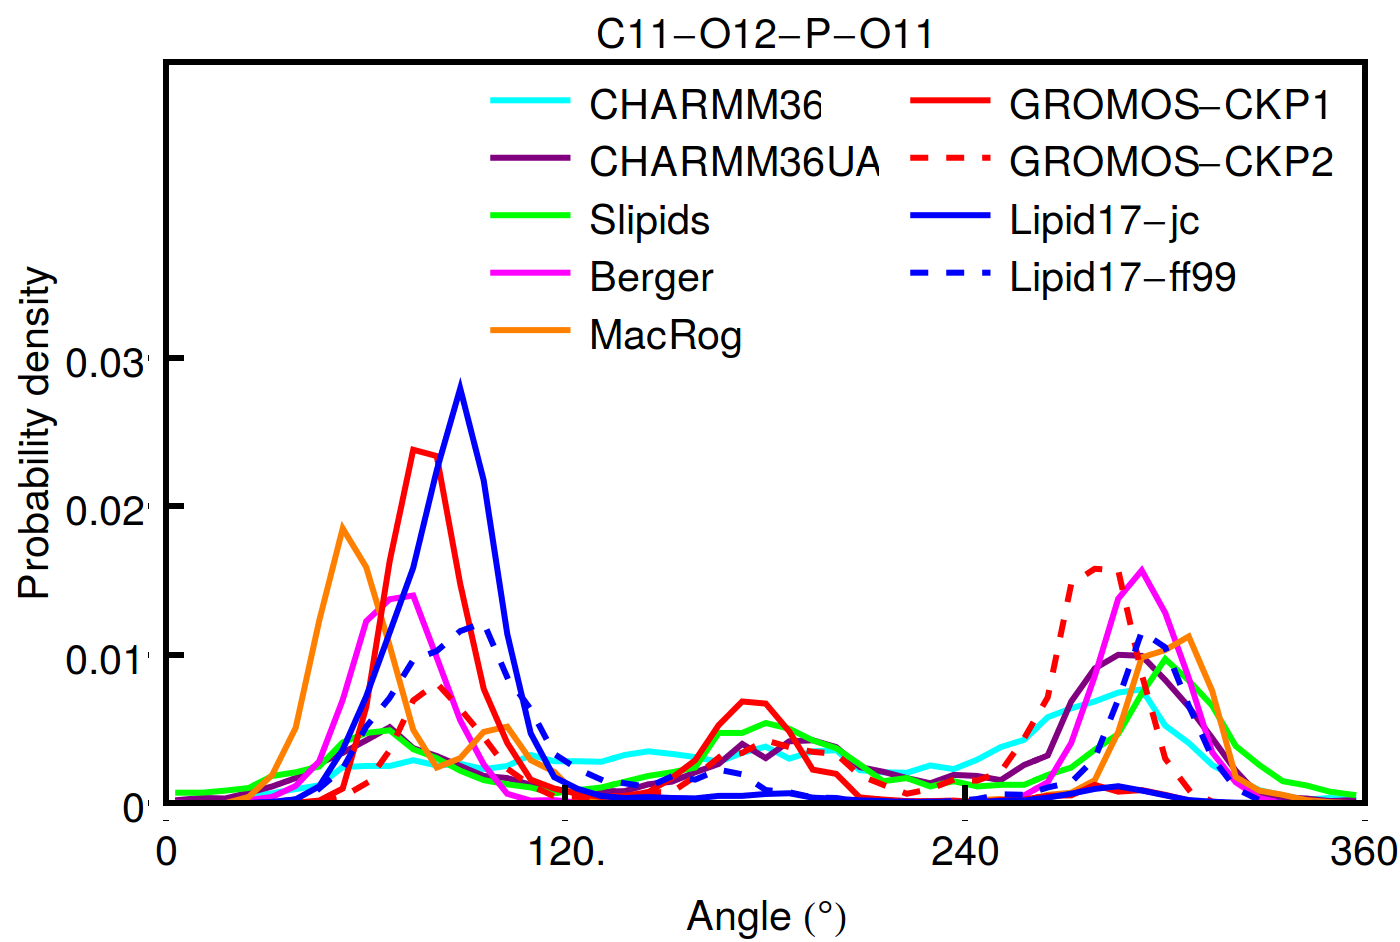
\includegraphics[width=8.0cm]{../Figs/diheds_pops8.png}
  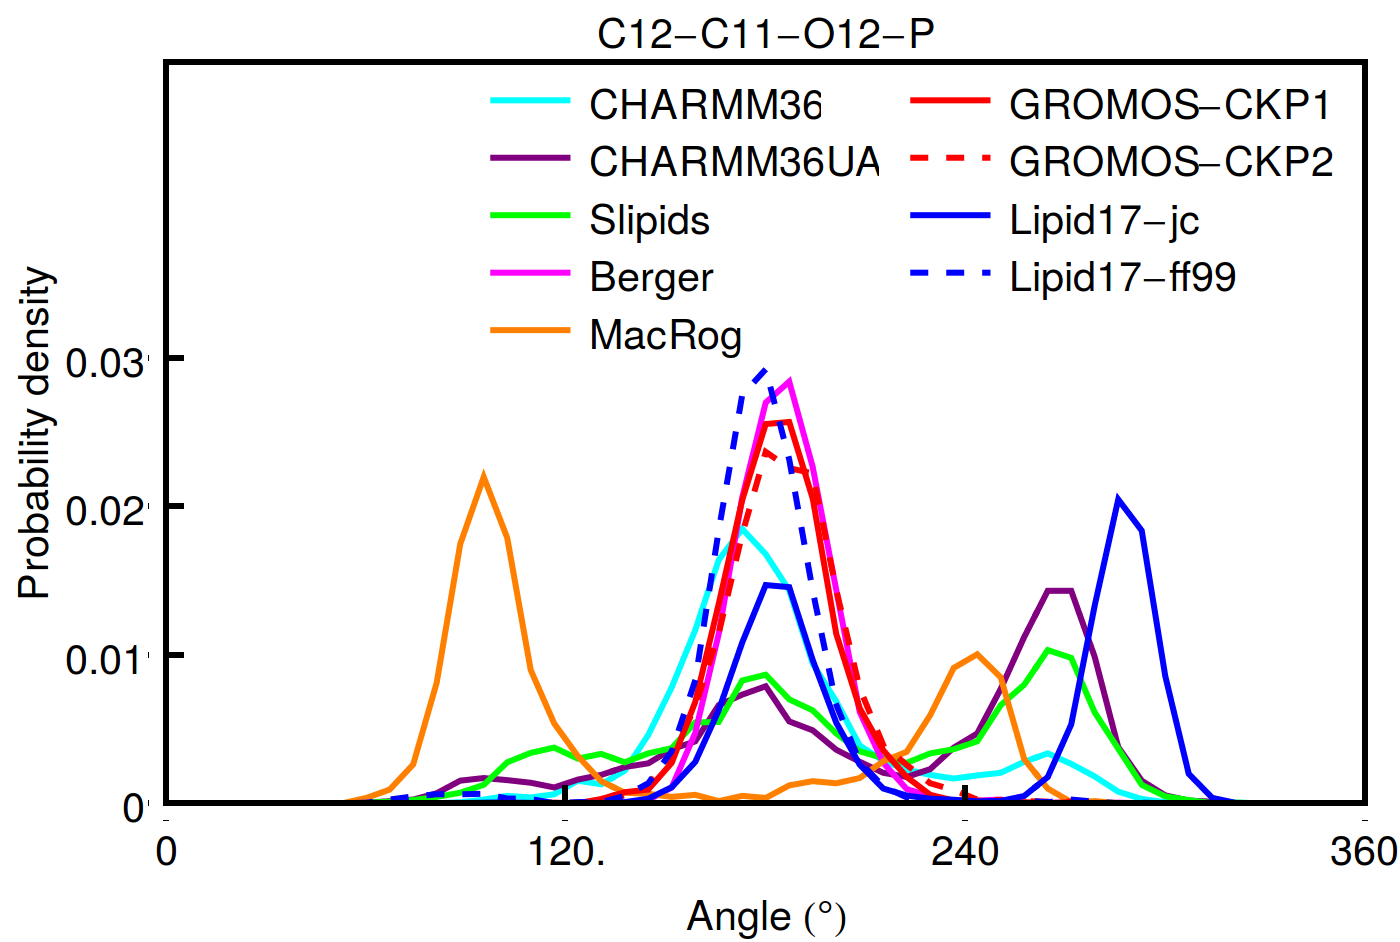
\includegraphics[width=8.0cm]{../Figs/diheds_pops9.png}
  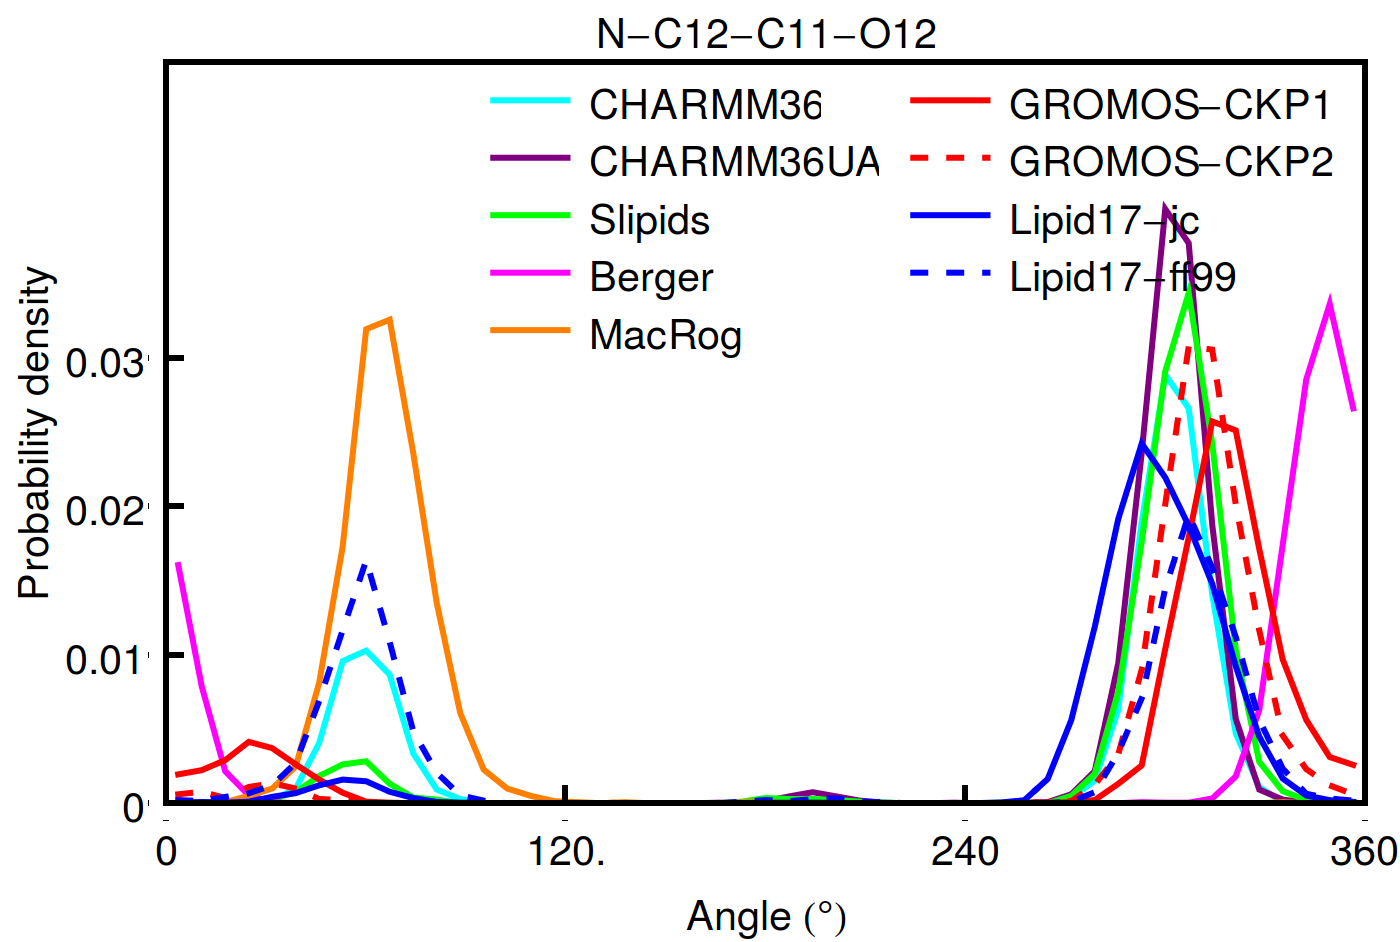
\includegraphics[width=8.0cm]{../Figs/diheds_pops10.png}
  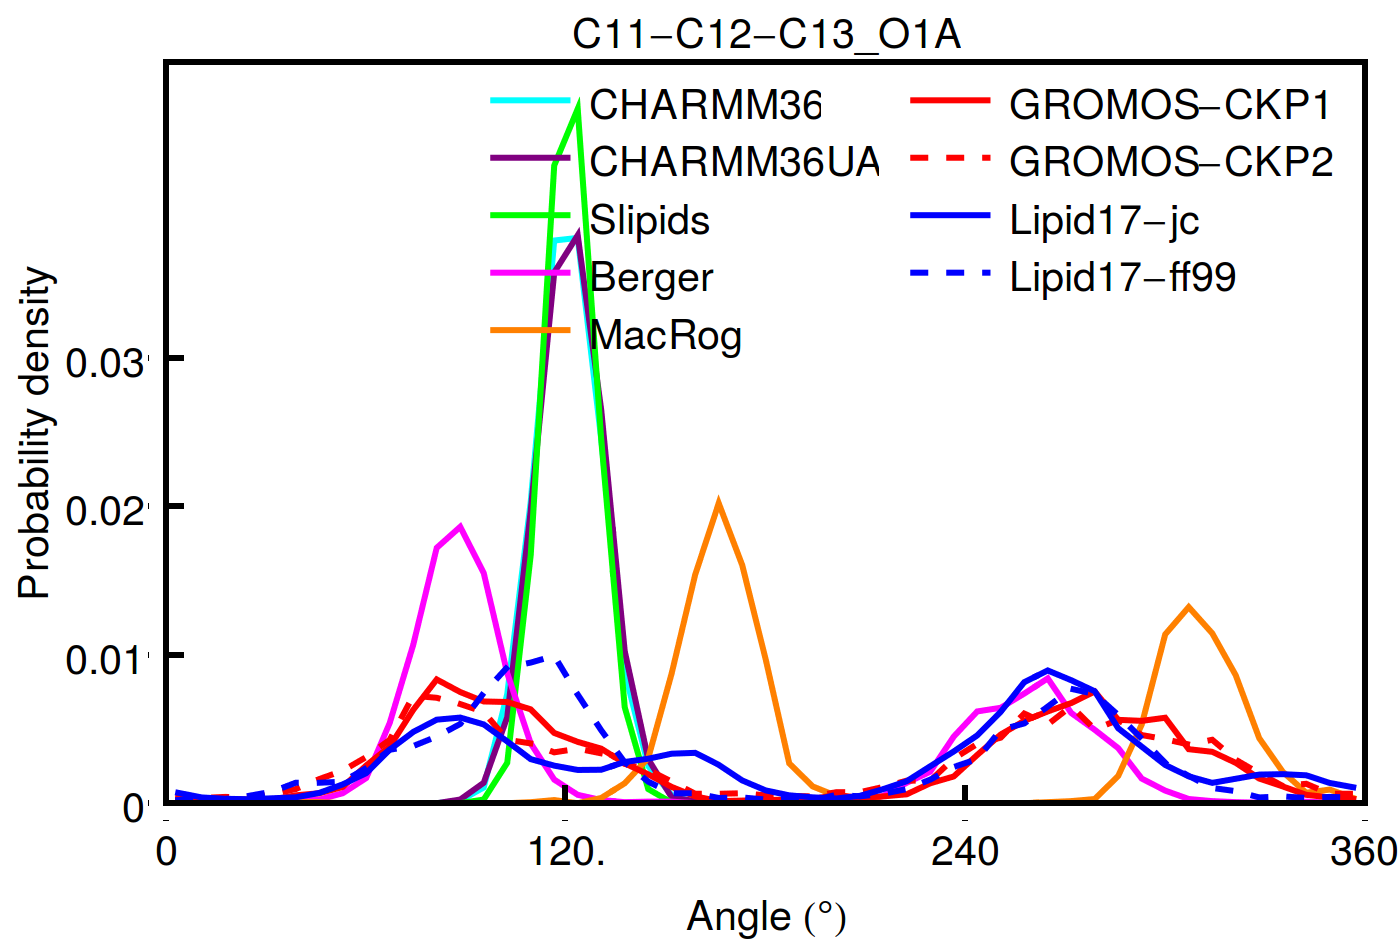
\includegraphics[width=8.0cm]{../Figs/diheds_pops11.png}
  \caption{\label{dihedralsHG}
    Dihedral angle distributions of bonds from phosphate to headgroup from different simulation models.
  }
\end{figure*}



\pagebreak
\section{Details of the rough subjective force field ranking (Fig.~\ref{comparisonTablePS})} 

The assessment was based fully on the Fig.~\ref{HGorderParametersPS}.
%
First, for each carbon (the columns in Fig.~\ref{HGorderParametersPS}) in each force field (the rows),
we looked separately at deviations in magnitude and forking.

{\bf Magnitude} deviations, i.e., how close to the experimentally obtained C--H order parameters (OPs)
the force-field-produced OPs were.
%
For each carbon, the following 5-step scale was used:
%
\begin{description}
\item [0 (~):] \noindent {More than half of all the calculated OPs (that is, of all different hydrogens in all different lipids) were within the {\it subjective sweet spots} (SSP, blue-shaded areas in Fig.~\ref{HGorderParametersPS}).}
%
\item [1 ({\textsf{\tiny M}}):] \noindent {All the calculated OPs  were $< 0.03$ units away from the SSP.}
%
\item [2  ({\textsf{\small M}}):] \noindent {All the calculated OPs  were $< 0.05$ units away from the SSP.}
%
\item [3 ({\textsf{\large M}}):] \noindent {All the calculated OPs  were $< 0.10$ units away from the SSP.}
%
\item [4 ({\textsf{\Large M}}):] \noindent {Some of the calculated OPs  were $> 0.10$ units  away from the SSP.}
\end{description}

{\bf Forking} deviations, i.e., how well the difference in order parameters of two hydrogens attached to a given carbon matched that obtained experimentally. Note that this is not relevant for $\beta$ and $\mathrm{g_2}$, which have only one hydrogen. For the $\alpha$ carbon,  for which a considerable forking of 0.105 is experimentally seen, the following 5-step scale was used:
\begin{description}
\item [0 (~):] \noindent {The distance $D$ between the dots (that mark the measurement-time-weighted averages in Fig.~\ref{HGorderParametersPS}) was $0.08 < D< 0.13$ units for all the calculated OPs (that is, for all different lipids).}
%
\item [1 ({\textsf{\tiny F}}):] \noindent {$(0.06 < D < 0.08)$ OR $(0.13 < D < 0.15)$.}
%
\item [2  ({\textsf{\small F}}):] \noindent {$(0.04 < D < 0.06)$ OR $(0.15 < D < 0.17)$.}
%
\item [3 ({\textsf{\large F}}):] \noindent {$(0.02 < D < 0.04)$ OR $(0.17 < D < 0.19)$.}
%
\item [4 ({\textsf{\Large F}}):] \noindent {$(D<0.02)$ OR $(0.19<D)$.}
\end{description}
%
For the $\mathrm{g_3}$ carbon, for which no forking is indicated by experiments, the following 5-step scale was used:
%
\begin{description}
\item [0 (~):] \noindent {$ D< 0.02$.}
%
\item [1 ({\textsf{\tiny F}}):] \noindent {$0.02 < D < 0.04$.}
%
\item [2  ({\textsf{\small F}}):] \noindent {$0.04 < D < 0.06$.}
%
\item [3 ({\textsf{\large F}}):] \noindent {$0.06 < D < 0.08$.}
%
\item [4 ({\textsf{\Large F}}):] \noindent {$0.08 < D$.}
\end{description}
%
For the $\mathrm{g_1}$ carbon, for which a considerable forking of 0.13 is experimentally seen, the following 5-step scale was used:
%
\begin{description}
\item [0 (~):] \noindent {$0.11 < D < 0.15$.}
%
\item [1 ({\textsf{\tiny F}}):] \noindent {$(0.09 < D < 0.11)$ OR $(0.15 < D < 0.17)$.}
%
\item [2  ({\textsf{\small F}}):] \noindent {$(0.07 < D < 0.09)$ OR $(0.17 < D < 0.19)$.}
%
\item [3 ({\textsf{\large F}}):] \noindent {$(0.05 < D < 0.07)$ OR $(0.19 < D < 0.21)$.}
%
\item [4 ({\textsf{\Large F}}):] \noindent {$(D<0.05)$ OR $(0.21<D)$.}
\end{description}

Based on these assessments of magnitude and forking deviations,
each carbon was then assigned to one of the following groups:
"within experimental error"
(magnitude and forking deviations both on step 0 of the scales described above),
"almost within experimental error"
(sum of the magnitude and forking deviation steps 1 or 2),
"clear deviation from experiments"
(sum of magnitude and forking deviation steps from 3 to 5), and
"major deviation from experiments"
(sum of magnitude and forking deviation steps from 6 to 8).
These groups are indicated by colors in Fig.~4.
(Note that for $\beta$ and $\mathrm{g_2}$, for which there can be no forking,
the corresponding group assigment limits were: 0, 1, 2, and 3.)

Finally, the total ability of the force field to describe the headgroup and
glycerol structure was estimated.
To this end, the groups were given the following weights:
0 (within experimental error),
1 (almost within experimental error),
2 (clear deviation from experiments),
4 (major deviation from experiments),
and the weights of the five carbons were summed up.
The sum, given in the $\Sigma$-column of Fig.~\ref{HGorderParametersPS},
was then used to (roughly and subjectively, as should be clear from the
above description) rank the force fields.

\newpage


% Create the reference section using BibTe
\bibliography{refs.bib}

%\newpage
%\section{APPENDIX: The NMR results reported by Tiago Ferreira}

\listoftodos

\end{document}
%
% ****** End of file aiptemplate.tex ******
